\documentclass[journal,10pt]{IEEEtran}

\usepackage[T1]{fontenc}
\usepackage{amsmath,amssymb,amsthm}
\usepackage{booktabs}
\usepackage{graphicx}
\usepackage{multirow}
\usepackage{algorithm2e}
\usepackage{tikz}
\usetikzlibrary{arrows.meta,positioning}
\usepackage{adjustbox}
\usepackage[backend=biber,style=ieee,sorting=none,maxnames=6]{biblatex}
\emergencystretch=2em

\newtheorem{proposition}{Proposition}
\newtheorem{lemma}{Lemma}
\newtheorem{theorem}{Theorem}
\definecolor{deepblue}{RGB}{81,132,178}
\definecolor{lightblue}{RGB}{170,212,248}
\definecolor{deeppink}{RGB}{213,82,118}
\definecolor{improvedpink}{RGB}{255,138,174}
\definecolor{inputyellow}{RGB}{255,248,154}
\definecolor{outputpink}{RGB}{255,178,166}
\tikzset{
  mod/.style={rectangle,rounded corners=2pt,draw=deepblue,fill=lightblue,minimum height=.65cm,align=center,font=\scriptsize},
  modimp/.style={rectangle,rounded corners=2pt,draw=deeppink,fill=improvedpink,minimum height=.65cm,align=center,font=\scriptsize},
  modin/.style={rectangle,draw=deepblue,fill=inputyellow,minimum height=.65cm,align=center,font=\scriptsize},
  modout/.style={rectangle,draw=deeppink,fill=outputpink,minimum height=.65cm,align=center,font=\scriptsize},
  flow/.style={-Stealth,thick,deepblue},
  flowimp/.style={-Stealth,thick,deeppink},
}

% Auto-generated by run_randomized_experiments.py; do not edit.
\newcommand{\RandCaseCount}{700}
\newcommand{\RandSeedCount}{100}
\newcommand{\RandCrossingBZeroSuccessPct}{86.0}
\newcommand{\RandCrossingBZeroReachPct}{100.0}
\newcommand{\RandCrossingBZeroCollisionPct}{14.0}
\newcommand{\RandCrossingBZeroStopPct}{0.0}
\newcommand{\RandCrossingBZeroClearance}{0.177}
\newcommand{\RandCrossingBZeroArrival}{9.00}
\newcommand{\RandCrossingBZeroProgressPct}{100.0}
\newcommand{\RandCrossingBZeroAvgSpeed}{3.44}
\newcommand{\RandCrossingBZeroJerkRms}{1.01}
\newcommand{\RandCrossingBZeroRuntimePfifty}{5.11}
\newcommand{\RandCrossingBZeroRuntimePninetyfive}{17.04}
\newcommand{\RandCrossingBZeroRuntimePninetynine}{52.02}
\newcommand{\RandCrossingBOneSuccessPct}{81.0}
\newcommand{\RandCrossingBOneReachPct}{86.0}
\newcommand{\RandCrossingBOneCollisionPct}{5.0}
\newcommand{\RandCrossingBOneStopPct}{14.0}
\newcommand{\RandCrossingBOneClearance}{0.512}
\newcommand{\RandCrossingBOneArrival}{9.00}
\newcommand{\RandCrossingBOneProgressPct}{91.7}
\newcommand{\RandCrossingBOneAvgSpeed}{3.16}
\newcommand{\RandCrossingBOneJerkRms}{1.08}
\newcommand{\RandCrossingBOneRuntimePfifty}{5.41}
\newcommand{\RandCrossingBOneRuntimePninetyfive}{36.65}
\newcommand{\RandCrossingBOneRuntimePninetynine}{73.60}
\newcommand{\RandCrossingBTwoSuccessPct}{89.0}
\newcommand{\RandCrossingBTwoReachPct}{100.0}
\newcommand{\RandCrossingBTwoCollisionPct}{11.0}
\newcommand{\RandCrossingBTwoStopPct}{0.0}
\newcommand{\RandCrossingBTwoClearance}{0.247}
\newcommand{\RandCrossingBTwoArrival}{9.00}
\newcommand{\RandCrossingBTwoProgressPct}{100.0}
\newcommand{\RandCrossingBTwoAvgSpeed}{3.44}
\newcommand{\RandCrossingBTwoJerkRms}{1.00}
\newcommand{\RandCrossingBTwoRuntimePfifty}{16.95}
\newcommand{\RandCrossingBTwoRuntimePninetyfive}{61.00}
\newcommand{\RandCrossingBTwoRuntimePninetynine}{157.46}
\newcommand{\RandCrossingMikuSuccessPct}{100.0}
\newcommand{\RandCrossingMikuReachPct}{100.0}
\newcommand{\RandCrossingMikuCollisionPct}{0.0}
\newcommand{\RandCrossingMikuStopPct}{0.0}
\newcommand{\RandCrossingMikuClearance}{0.259}
\newcommand{\RandCrossingMikuArrival}{9.00}
\newcommand{\RandCrossingMikuProgressPct}{100.0}
\newcommand{\RandCrossingMikuAvgSpeed}{3.44}
\newcommand{\RandCrossingMikuJerkRms}{1.07}
\newcommand{\RandCrossingMikuRuntimePfifty}{5.46}
\newcommand{\RandCrossingMikuRuntimePninetyfive}{24.25}
\newcommand{\RandCrossingMikuRuntimePninetynine}{31.92}
\newcommand{\RandCutInBZeroSuccessPct}{85.0}
\newcommand{\RandCutInBZeroReachPct}{88.0}
\newcommand{\RandCutInBZeroCollisionPct}{5.0}
\newcommand{\RandCutInBZeroStopPct}{12.0}
\newcommand{\RandCutInBZeroClearance}{2.494}
\newcommand{\RandCutInBZeroArrival}{10.00}
\newcommand{\RandCutInBZeroProgressPct}{98.4}
\newcommand{\RandCutInBZeroAvgSpeed}{4.04}
\newcommand{\RandCutInBZeroJerkRms}{0.53}
\newcommand{\RandCutInBZeroRuntimePfifty}{3.85}
\newcommand{\RandCutInBZeroRuntimePninetyfive}{24.12}
\newcommand{\RandCutInBZeroRuntimePninetynine}{47.98}
\newcommand{\RandCutInBOneSuccessPct}{83.0}
\newcommand{\RandCutInBOneReachPct}{86.0}
\newcommand{\RandCutInBOneCollisionPct}{5.0}
\newcommand{\RandCutInBOneStopPct}{14.0}
\newcommand{\RandCutInBOneClearance}{2.611}
\newcommand{\RandCutInBOneArrival}{10.00}
\newcommand{\RandCutInBOneProgressPct}{96.7}
\newcommand{\RandCutInBOneAvgSpeed}{3.97}
\newcommand{\RandCutInBOneJerkRms}{0.56}
\newcommand{\RandCutInBOneRuntimePfifty}{3.86}
\newcommand{\RandCutInBOneRuntimePninetyfive}{29.86}
\newcommand{\RandCutInBOneRuntimePninetynine}{73.82}
\newcommand{\RandCutInBTwoSuccessPct}{85.0}
\newcommand{\RandCutInBTwoReachPct}{88.0}
\newcommand{\RandCutInBTwoCollisionPct}{5.0}
\newcommand{\RandCutInBTwoStopPct}{12.0}
\newcommand{\RandCutInBTwoClearance}{2.532}
\newcommand{\RandCutInBTwoArrival}{10.00}
\newcommand{\RandCutInBTwoProgressPct}{97.8}
\newcommand{\RandCutInBTwoAvgSpeed}{4.01}
\newcommand{\RandCutInBTwoJerkRms}{0.55}
\newcommand{\RandCutInBTwoRuntimePfifty}{11.72}
\newcommand{\RandCutInBTwoRuntimePninetyfive}{79.45}
\newcommand{\RandCutInBTwoRuntimePninetynine}{150.34}
\newcommand{\RandCutInMikuSuccessPct}{82.0}
\newcommand{\RandCutInMikuReachPct}{82.0}
\newcommand{\RandCutInMikuCollisionPct}{0.0}
\newcommand{\RandCutInMikuStopPct}{18.0}
\newcommand{\RandCutInMikuClearance}{3.055}
\newcommand{\RandCutInMikuArrival}{10.00}
\newcommand{\RandCutInMikuProgressPct}{92.3}
\newcommand{\RandCutInMikuAvgSpeed}{3.79}
\newcommand{\RandCutInMikuJerkRms}{0.77}
\newcommand{\RandCutInMikuRuntimePfifty}{4.32}
\newcommand{\RandCutInMikuRuntimePninetyfive}{50.49}
\newcommand{\RandCutInMikuRuntimePninetynine}{95.60}
\newcommand{\RandParkedBZeroSuccessPct}{59.0}
\newcommand{\RandParkedBZeroReachPct}{59.0}
\newcommand{\RandParkedBZeroCollisionPct}{2.0}
\newcommand{\RandParkedBZeroStopPct}{41.0}
\newcommand{\RandParkedBZeroClearance}{0.335}
\newcommand{\RandParkedBZeroArrival}{10.00}
\newcommand{\RandParkedBZeroProgressPct}{72.1}
\newcommand{\RandParkedBZeroAvgSpeed}{3.39}
\newcommand{\RandParkedBZeroJerkRms}{1.23}
\newcommand{\RandParkedBZeroRuntimePfifty}{5.51}
\newcommand{\RandParkedBZeroRuntimePninetyfive}{89.96}
\newcommand{\RandParkedBZeroRuntimePninetynine}{195.58}
\newcommand{\RandParkedBOneSuccessPct}{52.0}
\newcommand{\RandParkedBOneReachPct}{52.0}
\newcommand{\RandParkedBOneCollisionPct}{2.0}
\newcommand{\RandParkedBOneStopPct}{48.0}
\newcommand{\RandParkedBOneClearance}{0.435}
\newcommand{\RandParkedBOneArrival}{10.00}
\newcommand{\RandParkedBOneProgressPct}{64.8}
\newcommand{\RandParkedBOneAvgSpeed}{3.05}
\newcommand{\RandParkedBOneJerkRms}{1.60}
\newcommand{\RandParkedBOneRuntimePfifty}{21.36}
\newcommand{\RandParkedBOneRuntimePninetyfive}{106.25}
\newcommand{\RandParkedBOneRuntimePninetynine}{198.81}
\newcommand{\RandParkedBTwoSuccessPct}{52.0}
\newcommand{\RandParkedBTwoReachPct}{52.0}
\newcommand{\RandParkedBTwoCollisionPct}{2.0}
\newcommand{\RandParkedBTwoStopPct}{48.0}
\newcommand{\RandParkedBTwoClearance}{0.435}
\newcommand{\RandParkedBTwoArrival}{10.00}
\newcommand{\RandParkedBTwoProgressPct}{64.8}
\newcommand{\RandParkedBTwoAvgSpeed}{3.05}
\newcommand{\RandParkedBTwoJerkRms}{1.60}
\newcommand{\RandParkedBTwoRuntimePfifty}{47.51}
\newcommand{\RandParkedBTwoRuntimePninetyfive}{246.06}
\newcommand{\RandParkedBTwoRuntimePninetynine}{397.85}
\newcommand{\RandParkedMikuSuccessPct}{67.0}
\newcommand{\RandParkedMikuReachPct}{67.0}
\newcommand{\RandParkedMikuCollisionPct}{0.0}
\newcommand{\RandParkedMikuStopPct}{33.0}
\newcommand{\RandParkedMikuClearance}{0.293}
\newcommand{\RandParkedMikuArrival}{10.00}
\newcommand{\RandParkedMikuProgressPct}{77.4}
\newcommand{\RandParkedMikuAvgSpeed}{3.64}
\newcommand{\RandParkedMikuJerkRms}{1.07}
\newcommand{\RandParkedMikuRuntimePfifty}{6.29}
\newcommand{\RandParkedMikuRuntimePninetyfive}{57.59}
\newcommand{\RandParkedMikuRuntimePninetynine}{71.15}
\newcommand{\RandNarrowBZeroSuccessPct}{1.0}
\newcommand{\RandNarrowBZeroReachPct}{1.0}
\newcommand{\RandNarrowBZeroCollisionPct}{0.0}
\newcommand{\RandNarrowBZeroStopPct}{99.0}
\newcommand{\RandNarrowBZeroClearance}{0.930}
\newcommand{\RandNarrowBZeroArrival}{12.00}
\newcommand{\RandNarrowBZeroProgressPct}{34.8}
\newcommand{\RandNarrowBZeroAvgSpeed}{1.13}
\newcommand{\RandNarrowBZeroJerkRms}{0.46}
\newcommand{\RandNarrowBZeroRuntimePfifty}{19.30}
\newcommand{\RandNarrowBZeroRuntimePninetyfive}{52.51}
\newcommand{\RandNarrowBZeroRuntimePninetynine}{71.62}
\newcommand{\RandNarrowBOneSuccessPct}{1.0}
\newcommand{\RandNarrowBOneReachPct}{1.0}
\newcommand{\RandNarrowBOneCollisionPct}{0.0}
\newcommand{\RandNarrowBOneStopPct}{99.0}
\newcommand{\RandNarrowBOneClearance}{0.956}
\newcommand{\RandNarrowBOneArrival}{12.00}
\newcommand{\RandNarrowBOneProgressPct}{34.8}
\newcommand{\RandNarrowBOneAvgSpeed}{1.13}
\newcommand{\RandNarrowBOneJerkRms}{0.46}
\newcommand{\RandNarrowBOneRuntimePfifty}{19.04}
\newcommand{\RandNarrowBOneRuntimePninetyfive}{52.16}
\newcommand{\RandNarrowBOneRuntimePninetynine}{71.69}
\newcommand{\RandNarrowBTwoSuccessPct}{1.0}
\newcommand{\RandNarrowBTwoReachPct}{1.0}
\newcommand{\RandNarrowBTwoCollisionPct}{0.0}
\newcommand{\RandNarrowBTwoStopPct}{99.0}
\newcommand{\RandNarrowBTwoClearance}{0.956}
\newcommand{\RandNarrowBTwoArrival}{12.00}
\newcommand{\RandNarrowBTwoProgressPct}{34.8}
\newcommand{\RandNarrowBTwoAvgSpeed}{1.13}
\newcommand{\RandNarrowBTwoJerkRms}{0.46}
\newcommand{\RandNarrowBTwoRuntimePfifty}{57.84}
\newcommand{\RandNarrowBTwoRuntimePninetyfive}{155.10}
\newcommand{\RandNarrowBTwoRuntimePninetynine}{217.84}
\newcommand{\RandNarrowMikuSuccessPct}{74.0}
\newcommand{\RandNarrowMikuReachPct}{74.0}
\newcommand{\RandNarrowMikuCollisionPct}{0.0}
\newcommand{\RandNarrowMikuStopPct}{26.0}
\newcommand{\RandNarrowMikuClearance}{0.476}
\newcommand{\RandNarrowMikuArrival}{12.00}
\newcommand{\RandNarrowMikuProgressPct}{82.7}
\newcommand{\RandNarrowMikuAvgSpeed}{2.69}
\newcommand{\RandNarrowMikuJerkRms}{0.25}
\newcommand{\RandNarrowMikuRuntimePfifty}{12.80}
\newcommand{\RandNarrowMikuRuntimePninetyfive}{31.43}
\newcommand{\RandNarrowMikuRuntimePninetynine}{68.00}
\newcommand{\RandInterleavedBZeroSuccessPct}{93.0}
\newcommand{\RandInterleavedBZeroReachPct}{100.0}
\newcommand{\RandInterleavedBZeroCollisionPct}{7.0}
\newcommand{\RandInterleavedBZeroStopPct}{0.0}
\newcommand{\RandInterleavedBZeroClearance}{0.099}
\newcommand{\RandInterleavedBZeroArrival}{14.00}
\newcommand{\RandInterleavedBZeroProgressPct}{100.0}
\newcommand{\RandInterleavedBZeroAvgSpeed}{3.14}
\newcommand{\RandInterleavedBZeroJerkRms}{0.91}
\newcommand{\RandInterleavedBZeroRuntimePfifty}{10.53}
\newcommand{\RandInterleavedBZeroRuntimePninetyfive}{40.20}
\newcommand{\RandInterleavedBZeroRuntimePninetynine}{75.22}
\newcommand{\RandInterleavedBOneSuccessPct}{74.0}
\newcommand{\RandInterleavedBOneReachPct}{77.0}
\newcommand{\RandInterleavedBOneCollisionPct}{3.0}
\newcommand{\RandInterleavedBOneStopPct}{23.0}
\newcommand{\RandInterleavedBOneClearance}{0.261}
\newcommand{\RandInterleavedBOneArrival}{14.00}
\newcommand{\RandInterleavedBOneProgressPct}{85.5}
\newcommand{\RandInterleavedBOneAvgSpeed}{2.69}
\newcommand{\RandInterleavedBOneJerkRms}{0.93}
\newcommand{\RandInterleavedBOneRuntimePfifty}{13.30}
\newcommand{\RandInterleavedBOneRuntimePninetyfive}{60.98}
\newcommand{\RandInterleavedBOneRuntimePninetynine}{77.56}
\newcommand{\RandInterleavedBTwoSuccessPct}{95.0}
\newcommand{\RandInterleavedBTwoReachPct}{100.0}
\newcommand{\RandInterleavedBTwoCollisionPct}{5.0}
\newcommand{\RandInterleavedBTwoStopPct}{0.0}
\newcommand{\RandInterleavedBTwoClearance}{0.128}
\newcommand{\RandInterleavedBTwoArrival}{14.00}
\newcommand{\RandInterleavedBTwoProgressPct}{100.0}
\newcommand{\RandInterleavedBTwoAvgSpeed}{3.14}
\newcommand{\RandInterleavedBTwoJerkRms}{0.92}
\newcommand{\RandInterleavedBTwoRuntimePfifty}{35.44}
\newcommand{\RandInterleavedBTwoRuntimePninetyfive}{125.87}
\newcommand{\RandInterleavedBTwoRuntimePninetynine}{226.48}
\newcommand{\RandInterleavedMikuSuccessPct}{90.0}
\newcommand{\RandInterleavedMikuReachPct}{90.0}
\newcommand{\RandInterleavedMikuCollisionPct}{0.0}
\newcommand{\RandInterleavedMikuStopPct}{10.0}
\newcommand{\RandInterleavedMikuClearance}{0.647}
\newcommand{\RandInterleavedMikuArrival}{14.00}
\newcommand{\RandInterleavedMikuProgressPct}{91.6}
\newcommand{\RandInterleavedMikuAvgSpeed}{2.88}
\newcommand{\RandInterleavedMikuJerkRms}{1.14}
\newcommand{\RandInterleavedMikuRuntimePfifty}{12.29}
\newcommand{\RandInterleavedMikuRuntimePninetyfive}{79.90}
\newcommand{\RandInterleavedMikuRuntimePninetynine}{100.56}
\newcommand{\RandNoiseBZeroSuccessPct}{33.0}
\newcommand{\RandNoiseBZeroReachPct}{46.0}
\newcommand{\RandNoiseBZeroCollisionPct}{14.0}
\newcommand{\RandNoiseBZeroStopPct}{54.0}
\newcommand{\RandNoiseBZeroClearance}{6.605}
\newcommand{\RandNoiseBZeroArrival}{10.00}
\newcommand{\RandNoiseBZeroProgressPct}{63.5}
\newcommand{\RandNoiseBZeroAvgSpeed}{2.60}
\newcommand{\RandNoiseBZeroJerkRms}{2.13}
\newcommand{\RandNoiseBZeroRuntimePfifty}{14.28}
\newcommand{\RandNoiseBZeroRuntimePninetyfive}{33.83}
\newcommand{\RandNoiseBZeroRuntimePninetynine}{47.21}
\newcommand{\RandNoiseBOneSuccessPct}{30.0}
\newcommand{\RandNoiseBOneReachPct}{42.0}
\newcommand{\RandNoiseBOneCollisionPct}{13.0}
\newcommand{\RandNoiseBOneStopPct}{58.0}
\newcommand{\RandNoiseBOneClearance}{6.772}
\newcommand{\RandNoiseBOneArrival}{10.00}
\newcommand{\RandNoiseBOneProgressPct}{61.5}
\newcommand{\RandNoiseBOneAvgSpeed}{2.52}
\newcommand{\RandNoiseBOneJerkRms}{2.15}
\newcommand{\RandNoiseBOneRuntimePfifty}{16.62}
\newcommand{\RandNoiseBOneRuntimePninetyfive}{33.79}
\newcommand{\RandNoiseBOneRuntimePninetynine}{47.66}
\newcommand{\RandNoiseBTwoSuccessPct}{33.0}
\newcommand{\RandNoiseBTwoReachPct}{46.0}
\newcommand{\RandNoiseBTwoCollisionPct}{14.0}
\newcommand{\RandNoiseBTwoStopPct}{54.0}
\newcommand{\RandNoiseBTwoClearance}{6.605}
\newcommand{\RandNoiseBTwoArrival}{10.00}
\newcommand{\RandNoiseBTwoProgressPct}{63.5}
\newcommand{\RandNoiseBTwoAvgSpeed}{2.60}
\newcommand{\RandNoiseBTwoJerkRms}{2.13}
\newcommand{\RandNoiseBTwoRuntimePfifty}{36.45}
\newcommand{\RandNoiseBTwoRuntimePninetyfive}{68.84}
\newcommand{\RandNoiseBTwoRuntimePninetynine}{95.94}
\newcommand{\RandNoiseMikuSuccessPct}{17.0}
\newcommand{\RandNoiseMikuReachPct}{17.0}
\newcommand{\RandNoiseMikuCollisionPct}{0.0}
\newcommand{\RandNoiseMikuStopPct}{83.0}
\newcommand{\RandNoiseMikuClearance}{9.690}
\newcommand{\RandNoiseMikuArrival}{10.00}
\newcommand{\RandNoiseMikuProgressPct}{36.8}
\newcommand{\RandNoiseMikuAvgSpeed}{1.51}
\newcommand{\RandNoiseMikuJerkRms}{3.35}
\newcommand{\RandNoiseMikuRuntimePfifty}{19.47}
\newcommand{\RandNoiseMikuRuntimePninetyfive}{43.87}
\newcommand{\RandNoiseMikuRuntimePninetynine}{62.79}
\newcommand{\RandDelayedBZeroSuccessPct}{65.0}
\newcommand{\RandDelayedBZeroReachPct}{67.0}
\newcommand{\RandDelayedBZeroCollisionPct}{5.0}
\newcommand{\RandDelayedBZeroStopPct}{33.0}
\newcommand{\RandDelayedBZeroClearance}{0.136}
\newcommand{\RandDelayedBZeroArrival}{9.00}
\newcommand{\RandDelayedBZeroProgressPct}{85.8}
\newcommand{\RandDelayedBZeroAvgSpeed}{3.15}
\newcommand{\RandDelayedBZeroJerkRms}{2.06}
\newcommand{\RandDelayedBZeroRuntimePfifty}{15.99}
\newcommand{\RandDelayedBZeroRuntimePninetyfive}{76.56}
\newcommand{\RandDelayedBZeroRuntimePninetynine}{468.76}
\newcommand{\RandDelayedBOneSuccessPct}{37.0}
\newcommand{\RandDelayedBOneReachPct}{38.0}
\newcommand{\RandDelayedBOneCollisionPct}{4.0}
\newcommand{\RandDelayedBOneStopPct}{62.0}
\newcommand{\RandDelayedBOneClearance}{0.208}
\newcommand{\RandDelayedBOneArrival}{9.00}
\newcommand{\RandDelayedBOneProgressPct}{70.5}
\newcommand{\RandDelayedBOneAvgSpeed}{2.59}
\newcommand{\RandDelayedBOneJerkRms}{2.06}
\newcommand{\RandDelayedBOneRuntimePfifty}{23.73}
\newcommand{\RandDelayedBOneRuntimePninetyfive}{142.59}
\newcommand{\RandDelayedBOneRuntimePninetynine}{912.67}
\newcommand{\RandDelayedBTwoSuccessPct}{65.0}
\newcommand{\RandDelayedBTwoReachPct}{68.0}
\newcommand{\RandDelayedBTwoCollisionPct}{6.0}
\newcommand{\RandDelayedBTwoStopPct}{32.0}
\newcommand{\RandDelayedBTwoClearance}{0.178}
\newcommand{\RandDelayedBTwoArrival}{9.00}
\newcommand{\RandDelayedBTwoProgressPct}{86.0}
\newcommand{\RandDelayedBTwoAvgSpeed}{3.15}
\newcommand{\RandDelayedBTwoJerkRms}{2.14}
\newcommand{\RandDelayedBTwoRuntimePfifty}{67.75}
\newcommand{\RandDelayedBTwoRuntimePninetyfive}{257.08}
\newcommand{\RandDelayedBTwoRuntimePninetynine}{1825.01}
\newcommand{\RandDelayedMikuSuccessPct}{87.0}
\newcommand{\RandDelayedMikuReachPct}{87.0}
\newcommand{\RandDelayedMikuCollisionPct}{3.0}
\newcommand{\RandDelayedMikuStopPct}{13.0}
\newcommand{\RandDelayedMikuClearance}{0.179}
\newcommand{\RandDelayedMikuArrival}{8.64}
\newcommand{\RandDelayedMikuProgressPct}{94.1}
\newcommand{\RandDelayedMikuAvgSpeed}{3.64}
\newcommand{\RandDelayedMikuJerkRms}{1.79}
\newcommand{\RandDelayedMikuRuntimePfifty}{24.96}
\newcommand{\RandDelayedMikuRuntimePninetyfive}{239.72}
\newcommand{\RandDelayedMikuRuntimePninetynine}{493.93}
\newcommand{\RandAllBZeroSuccessPct}{60.3}
\newcommand{\RandAllBZeroReachPct}{65.9}
\newcommand{\RandAllBZeroCollisionPct}{6.7}
\newcommand{\RandAllBZeroStopPct}{34.1}
\newcommand{\RandAllBZeroClearance}{1.539}
\newcommand{\RandAllBZeroArrival}{10.53}
\newcommand{\RandAllBZeroProgressPct}{79.2}
\newcommand{\RandAllBZeroAvgSpeed}{2.98}
\newcommand{\RandAllBZeroJerkRms}{1.19}
\newcommand{\RandAllBZeroRuntimePfifty}{10.31}
\newcommand{\RandAllBZeroRuntimePninetyfive}{54.28}
\newcommand{\RandAllBZeroRuntimePninetynine}{117.89}
\newcommand{\RandAllBOneSuccessPct}{51.1}
\newcommand{\RandAllBOneReachPct}{54.6}
\newcommand{\RandAllBOneCollisionPct}{4.6}
\newcommand{\RandAllBOneStopPct}{45.4}
\newcommand{\RandAllBOneClearance}{1.679}
\newcommand{\RandAllBOneArrival}{10.50}
\newcommand{\RandAllBOneProgressPct}{72.2}
\newcommand{\RandAllBOneAvgSpeed}{2.73}
\newcommand{\RandAllBOneJerkRms}{1.26}
\newcommand{\RandAllBOneRuntimePfifty}{12.27}
\newcommand{\RandAllBOneRuntimePninetyfive}{68.37}
\newcommand{\RandAllBOneRuntimePninetynine}{146.73}
\newcommand{\RandAllBTwoSuccessPct}{60.0}
\newcommand{\RandAllBTwoReachPct}{65.0}
\newcommand{\RandAllBTwoCollisionPct}{6.1}
\newcommand{\RandAllBTwoStopPct}{35.0}
\newcommand{\RandAllBTwoClearance}{1.583}
\newcommand{\RandAllBTwoArrival}{10.54}
\newcommand{\RandAllBTwoProgressPct}{78.1}
\newcommand{\RandAllBTwoAvgSpeed}{2.93}
\newcommand{\RandAllBTwoJerkRms}{1.26}
\newcommand{\RandAllBTwoRuntimePfifty}{34.33}
\newcommand{\RandAllBTwoRuntimePninetyfive}{164.23}
\newcommand{\RandAllBTwoRuntimePninetynine}{391.91}
\newcommand{\RandAllMikuSuccessPct}{73.9}
\newcommand{\RandAllMikuReachPct}{73.9}
\newcommand{\RandAllMikuCollisionPct}{0.4}
\newcommand{\RandAllMikuStopPct}{26.1}
\newcommand{\RandAllMikuClearance}{2.086}
\newcommand{\RandAllMikuArrival}{10.56}
\newcommand{\RandAllMikuProgressPct}{82.1}
\newcommand{\RandAllMikuAvgSpeed}{3.08}
\newcommand{\RandAllMikuJerkRms}{1.35}
\newcommand{\RandAllMikuRuntimePfifty}{12.38}
\newcommand{\RandAllMikuRuntimePninetyfive}{61.64}
\newcommand{\RandAllMikuRuntimePninetynine}{237.95}
\newcommand{\RandCrossingMikuVsBZeroSuccessDiff}{14.0}
\newcommand{\RandCrossingMikuVsBZeroSuccessCiLow}{8.0}
\newcommand{\RandCrossingMikuVsBZeroSuccessCiHigh}{21.0}
\newcommand{\RandCrossingMikuVsBZeroSuccessEffect}{0.401}
\newcommand{\RandCrossingMikuVsBZeroSuccessMcNemarP}{0.0001221}
\newcommand{\RandCrossingMikuVsBZeroCollisionDiff}{-14.0}
\newcommand{\RandCrossingMikuVsBZeroCollisionCiLow}{-21.0}
\newcommand{\RandCrossingMikuVsBZeroCollisionCiHigh}{-8.0}
\newcommand{\RandCrossingMikuVsBZeroCollisionEffect}{-0.401}
\newcommand{\RandCrossingMikuVsBZeroCollisionMcNemarP}{0.0001221}
\newcommand{\RandCrossingMikuVsBZeroClearanceDiff}{0.082}
\newcommand{\RandCrossingMikuVsBZeroClearanceCiLow}{0.071}
\newcommand{\RandCrossingMikuVsBZeroClearanceCiHigh}{0.095}
\newcommand{\RandCrossingMikuVsBZeroClearanceEffect}{1.332}
\newcommand{\RandCrossingMikuVsBZeroTravelDiff}{-0.70}
\newcommand{\RandCrossingMikuVsBZeroTravelCiLow}{-1.05}
\newcommand{\RandCrossingMikuVsBZeroTravelCiHigh}{-0.35}
\newcommand{\RandCrossingMikuVsBZeroTravelEffect}{-0.401}
\newcommand{\RandCrossingMikuVsBZeroRuntimeDiff}{0.26}
\newcommand{\RandCrossingMikuVsBZeroRuntimeCiLow}{-0.64}
\newcommand{\RandCrossingMikuVsBZeroRuntimeCiHigh}{1.04}
\newcommand{\RandCrossingMikuVsBZeroRuntimeEffect}{0.060}
\newcommand{\RandCrossingMikuVsBOneSuccessDiff}{19.0}
\newcommand{\RandCrossingMikuVsBOneSuccessCiLow}{12.0}
\newcommand{\RandCrossingMikuVsBOneSuccessCiHigh}{27.0}
\newcommand{\RandCrossingMikuVsBOneSuccessEffect}{0.482}
\newcommand{\RandCrossingMikuVsBOneSuccessMcNemarP}{3.815e-06}
\newcommand{\RandCrossingMikuVsBOneCollisionDiff}{-5.0}
\newcommand{\RandCrossingMikuVsBOneCollisionCiLow}{-10.0}
\newcommand{\RandCrossingMikuVsBOneCollisionCiHigh}{-1.0}
\newcommand{\RandCrossingMikuVsBOneCollisionEffect}{-0.228}
\newcommand{\RandCrossingMikuVsBOneCollisionMcNemarP}{0.0625}
\newcommand{\RandCrossingMikuVsBOneClearanceDiff}{-0.253}
\newcommand{\RandCrossingMikuVsBOneClearanceCiLow}{-0.379}
\newcommand{\RandCrossingMikuVsBOneClearanceCiHigh}{-0.132}
\newcommand{\RandCrossingMikuVsBOneClearanceEffect}{-0.401}
\newcommand{\RandCrossingMikuVsBOneTravelDiff}{-0.95}
\newcommand{\RandCrossingMikuVsBOneTravelCiLow}{-1.35}
\newcommand{\RandCrossingMikuVsBOneTravelCiHigh}{-0.60}
\newcommand{\RandCrossingMikuVsBOneTravelEffect}{-0.482}
\newcommand{\RandCrossingMikuVsBOneRuntimeDiff}{-2.83}
\newcommand{\RandCrossingMikuVsBOneRuntimeCiLow}{-5.09}
\newcommand{\RandCrossingMikuVsBOneRuntimeCiHigh}{-0.89}
\newcommand{\RandCrossingMikuVsBOneRuntimeEffect}{-0.260}
\newcommand{\RandCrossingMikuVsBTwoSuccessDiff}{11.0}
\newcommand{\RandCrossingMikuVsBTwoSuccessCiLow}{5.0}
\newcommand{\RandCrossingMikuVsBTwoSuccessCiHigh}{18.0}
\newcommand{\RandCrossingMikuVsBTwoSuccessEffect}{0.350}
\newcommand{\RandCrossingMikuVsBTwoSuccessMcNemarP}{0.0009766}
\newcommand{\RandCrossingMikuVsBTwoCollisionDiff}{-11.0}
\newcommand{\RandCrossingMikuVsBTwoCollisionCiLow}{-18.0}
\newcommand{\RandCrossingMikuVsBTwoCollisionCiHigh}{-5.0}
\newcommand{\RandCrossingMikuVsBTwoCollisionEffect}{-0.350}
\newcommand{\RandCrossingMikuVsBTwoCollisionMcNemarP}{0.0009766}
\newcommand{\RandCrossingMikuVsBTwoClearanceDiff}{0.012}
\newcommand{\RandCrossingMikuVsBTwoClearanceCiLow}{-0.020}
\newcommand{\RandCrossingMikuVsBTwoClearanceCiHigh}{0.041}
\newcommand{\RandCrossingMikuVsBTwoClearanceEffect}{0.074}
\newcommand{\RandCrossingMikuVsBTwoTravelDiff}{-0.55}
\newcommand{\RandCrossingMikuVsBTwoTravelCiLow}{-0.85}
\newcommand{\RandCrossingMikuVsBTwoTravelCiHigh}{-0.25}
\newcommand{\RandCrossingMikuVsBTwoTravelEffect}{-0.350}
\newcommand{\RandCrossingMikuVsBTwoRuntimeDiff}{-17.78}
\newcommand{\RandCrossingMikuVsBTwoRuntimeCiLow}{-22.63}
\newcommand{\RandCrossingMikuVsBTwoRuntimeCiHigh}{-13.90}
\newcommand{\RandCrossingMikuVsBTwoRuntimeEffect}{-0.787}
\newcommand{\RandCutInMikuVsBZeroSuccessDiff}{-3.0}
\newcommand{\RandCutInMikuVsBZeroSuccessCiLow}{-7.0}
\newcommand{\RandCutInMikuVsBZeroSuccessCiHigh}{0.0}
\newcommand{\RandCutInMikuVsBZeroSuccessEffect}{-0.175}
\newcommand{\RandCutInMikuVsBZeroSuccessMcNemarP}{0.25}
\newcommand{\RandCutInMikuVsBZeroCollisionDiff}{-5.0}
\newcommand{\RandCutInMikuVsBZeroCollisionCiLow}{-9.0}
\newcommand{\RandCutInMikuVsBZeroCollisionCiHigh}{-1.0}
\newcommand{\RandCutInMikuVsBZeroCollisionEffect}{-0.228}
\newcommand{\RandCutInMikuVsBZeroCollisionMcNemarP}{0.0625}
\newcommand{\RandCutInMikuVsBZeroClearanceDiff}{0.560}
\newcommand{\RandCutInMikuVsBZeroClearanceCiLow}{0.209}
\newcommand{\RandCutInMikuVsBZeroClearanceCiHigh}{0.985}
\newcommand{\RandCutInMikuVsBZeroClearanceEffect}{0.281}
\newcommand{\RandCutInMikuVsBZeroTravelDiff}{0.15}
\newcommand{\RandCutInMikuVsBZeroTravelCiLow}{0.00}
\newcommand{\RandCutInMikuVsBZeroTravelCiHigh}{0.35}
\newcommand{\RandCutInMikuVsBZeroTravelEffect}{0.175}
\newcommand{\RandCutInMikuVsBZeroRuntimeDiff}{5.98}
\newcommand{\RandCutInMikuVsBZeroRuntimeCiLow}{2.79}
\newcommand{\RandCutInMikuVsBZeroRuntimeCiHigh}{10.60}
\newcommand{\RandCutInMikuVsBZeroRuntimeEffect}{0.287}
\newcommand{\RandCutInMikuVsBOneSuccessDiff}{-1.0}
\newcommand{\RandCutInMikuVsBOneSuccessCiLow}{-5.0}
\newcommand{\RandCutInMikuVsBOneSuccessCiHigh}{3.0}
\newcommand{\RandCutInMikuVsBOneSuccessEffect}{-0.045}
\newcommand{\RandCutInMikuVsBOneSuccessMcNemarP}{1}
\newcommand{\RandCutInMikuVsBOneCollisionDiff}{-5.0}
\newcommand{\RandCutInMikuVsBOneCollisionCiLow}{-9.0}
\newcommand{\RandCutInMikuVsBOneCollisionCiHigh}{-1.0}
\newcommand{\RandCutInMikuVsBOneCollisionEffect}{-0.228}
\newcommand{\RandCutInMikuVsBOneCollisionMcNemarP}{0.0625}
\newcommand{\RandCutInMikuVsBOneClearanceDiff}{0.444}
\newcommand{\RandCutInMikuVsBOneClearanceCiLow}{0.054}
\newcommand{\RandCutInMikuVsBOneClearanceCiHigh}{0.880}
\newcommand{\RandCutInMikuVsBOneClearanceEffect}{0.208}
\newcommand{\RandCutInMikuVsBOneTravelDiff}{0.05}
\newcommand{\RandCutInMikuVsBOneTravelCiLow}{-0.15}
\newcommand{\RandCutInMikuVsBOneTravelCiHigh}{0.30}
\newcommand{\RandCutInMikuVsBOneTravelEffect}{0.045}
\newcommand{\RandCutInMikuVsBOneRuntimeDiff}{5.29}
\newcommand{\RandCutInMikuVsBOneRuntimeCiLow}{2.33}
\newcommand{\RandCutInMikuVsBOneRuntimeCiHigh}{9.79}
\newcommand{\RandCutInMikuVsBOneRuntimeEffect}{0.259}
\newcommand{\RandCutInMikuVsBTwoSuccessDiff}{-3.0}
\newcommand{\RandCutInMikuVsBTwoSuccessCiLow}{-7.0}
\newcommand{\RandCutInMikuVsBTwoSuccessCiHigh}{0.0}
\newcommand{\RandCutInMikuVsBTwoSuccessEffect}{-0.175}
\newcommand{\RandCutInMikuVsBTwoSuccessMcNemarP}{0.25}
\newcommand{\RandCutInMikuVsBTwoCollisionDiff}{-5.0}
\newcommand{\RandCutInMikuVsBTwoCollisionCiLow}{-10.0}
\newcommand{\RandCutInMikuVsBTwoCollisionCiHigh}{-1.0}
\newcommand{\RandCutInMikuVsBTwoCollisionEffect}{-0.228}
\newcommand{\RandCutInMikuVsBTwoCollisionMcNemarP}{0.0625}
\newcommand{\RandCutInMikuVsBTwoClearanceDiff}{0.523}
\newcommand{\RandCutInMikuVsBTwoClearanceCiLow}{0.163}
\newcommand{\RandCutInMikuVsBTwoClearanceCiHigh}{0.949}
\newcommand{\RandCutInMikuVsBTwoClearanceEffect}{0.256}
\newcommand{\RandCutInMikuVsBTwoTravelDiff}{0.15}
\newcommand{\RandCutInMikuVsBTwoTravelCiLow}{0.00}
\newcommand{\RandCutInMikuVsBTwoTravelCiHigh}{0.35}
\newcommand{\RandCutInMikuVsBTwoTravelEffect}{0.175}
\newcommand{\RandCutInMikuVsBTwoRuntimeDiff}{-14.02}
\newcommand{\RandCutInMikuVsBTwoRuntimeCiLow}{-18.63}
\newcommand{\RandCutInMikuVsBTwoRuntimeCiHigh}{-10.50}
\newcommand{\RandCutInMikuVsBTwoRuntimeEffect}{-0.657}
\newcommand{\RandParkedMikuVsBZeroSuccessDiff}{8.0}
\newcommand{\RandParkedMikuVsBZeroSuccessCiLow}{3.0}
\newcommand{\RandParkedMikuVsBZeroSuccessCiHigh}{14.0}
\newcommand{\RandParkedMikuVsBZeroSuccessEffect}{0.293}
\newcommand{\RandParkedMikuVsBZeroSuccessMcNemarP}{0.007812}
\newcommand{\RandParkedMikuVsBZeroCollisionDiff}{-2.0}
\newcommand{\RandParkedMikuVsBZeroCollisionCiLow}{-5.0}
\newcommand{\RandParkedMikuVsBZeroCollisionCiHigh}{0.0}
\newcommand{\RandParkedMikuVsBZeroCollisionEffect}{-0.142}
\newcommand{\RandParkedMikuVsBZeroCollisionMcNemarP}{0.5}
\newcommand{\RandParkedMikuVsBZeroClearanceDiff}{-0.042}
\newcommand{\RandParkedMikuVsBZeroClearanceCiLow}{-0.077}
\newcommand{\RandParkedMikuVsBZeroClearanceCiHigh}{-0.001}
\newcommand{\RandParkedMikuVsBZeroClearanceEffect}{-0.220}
\newcommand{\RandParkedMikuVsBZeroTravelDiff}{-0.40}
\newcommand{\RandParkedMikuVsBZeroTravelCiLow}{-0.70}
\newcommand{\RandParkedMikuVsBZeroTravelCiHigh}{-0.15}
\newcommand{\RandParkedMikuVsBZeroTravelEffect}{-0.293}
\newcommand{\RandParkedMikuVsBZeroRuntimeDiff}{-11.29}
\newcommand{\RandParkedMikuVsBZeroRuntimeCiLow}{-22.51}
\newcommand{\RandParkedMikuVsBZeroRuntimeCiHigh}{-3.73}
\newcommand{\RandParkedMikuVsBZeroRuntimeEffect}{-0.219}
\newcommand{\RandParkedMikuVsBOneSuccessDiff}{15.0}
\newcommand{\RandParkedMikuVsBOneSuccessCiLow}{8.0}
\newcommand{\RandParkedMikuVsBOneSuccessCiHigh}{22.0}
\newcommand{\RandParkedMikuVsBOneSuccessEffect}{0.418}
\newcommand{\RandParkedMikuVsBOneSuccessMcNemarP}{6.104e-05}
\newcommand{\RandParkedMikuVsBOneCollisionDiff}{-2.0}
\newcommand{\RandParkedMikuVsBOneCollisionCiLow}{-5.0}
\newcommand{\RandParkedMikuVsBOneCollisionCiHigh}{0.0}
\newcommand{\RandParkedMikuVsBOneCollisionEffect}{-0.142}
\newcommand{\RandParkedMikuVsBOneCollisionMcNemarP}{0.5}
\newcommand{\RandParkedMikuVsBOneClearanceDiff}{-0.142}
\newcommand{\RandParkedMikuVsBOneClearanceCiLow}{-0.206}
\newcommand{\RandParkedMikuVsBOneClearanceCiHigh}{-0.079}
\newcommand{\RandParkedMikuVsBOneClearanceEffect}{-0.439}
\newcommand{\RandParkedMikuVsBOneTravelDiff}{-0.75}
\newcommand{\RandParkedMikuVsBOneTravelCiLow}{-1.10}
\newcommand{\RandParkedMikuVsBOneTravelCiHigh}{-0.40}
\newcommand{\RandParkedMikuVsBOneTravelEffect}{-0.418}
\newcommand{\RandParkedMikuVsBOneRuntimeDiff}{-14.65}
\newcommand{\RandParkedMikuVsBOneRuntimeCiLow}{-26.41}
\newcommand{\RandParkedMikuVsBOneRuntimeCiHigh}{-6.63}
\newcommand{\RandParkedMikuVsBOneRuntimeEffect}{-0.278}
\newcommand{\RandParkedMikuVsBTwoSuccessDiff}{15.0}
\newcommand{\RandParkedMikuVsBTwoSuccessCiLow}{8.0}
\newcommand{\RandParkedMikuVsBTwoSuccessCiHigh}{22.0}
\newcommand{\RandParkedMikuVsBTwoSuccessEffect}{0.418}
\newcommand{\RandParkedMikuVsBTwoSuccessMcNemarP}{6.104e-05}
\newcommand{\RandParkedMikuVsBTwoCollisionDiff}{-2.0}
\newcommand{\RandParkedMikuVsBTwoCollisionCiLow}{-5.0}
\newcommand{\RandParkedMikuVsBTwoCollisionCiHigh}{0.0}
\newcommand{\RandParkedMikuVsBTwoCollisionEffect}{-0.142}
\newcommand{\RandParkedMikuVsBTwoCollisionMcNemarP}{0.5}
\newcommand{\RandParkedMikuVsBTwoClearanceDiff}{-0.142}
\newcommand{\RandParkedMikuVsBTwoClearanceCiLow}{-0.208}
\newcommand{\RandParkedMikuVsBTwoClearanceCiHigh}{-0.080}
\newcommand{\RandParkedMikuVsBTwoClearanceEffect}{-0.439}
\newcommand{\RandParkedMikuVsBTwoTravelDiff}{-0.75}
\newcommand{\RandParkedMikuVsBTwoTravelCiLow}{-1.10}
\newcommand{\RandParkedMikuVsBTwoTravelCiHigh}{-0.40}
\newcommand{\RandParkedMikuVsBTwoTravelEffect}{-0.418}
\newcommand{\RandParkedMikuVsBTwoRuntimeDiff}{-64.29}
\newcommand{\RandParkedMikuVsBTwoRuntimeCiLow}{-89.88}
\newcommand{\RandParkedMikuVsBTwoRuntimeCiHigh}{-45.16}
\newcommand{\RandParkedMikuVsBTwoRuntimeEffect}{-0.550}
\newcommand{\RandNarrowMikuVsBZeroSuccessDiff}{73.0}
\newcommand{\RandNarrowMikuVsBZeroSuccessCiLow}{64.0}
\newcommand{\RandNarrowMikuVsBZeroSuccessCiHigh}{82.0}
\newcommand{\RandNarrowMikuVsBZeroSuccessEffect}{1.636}
\newcommand{\RandNarrowMikuVsBZeroSuccessMcNemarP}{2.118e-22}
\newcommand{\RandNarrowMikuVsBZeroCollisionDiff}{0.0}
\newcommand{\RandNarrowMikuVsBZeroCollisionCiLow}{0.0}
\newcommand{\RandNarrowMikuVsBZeroCollisionCiHigh}{0.0}
\newcommand{\RandNarrowMikuVsBZeroCollisionEffect}{0.000}
\newcommand{\RandNarrowMikuVsBZeroCollisionMcNemarP}{1}
\newcommand{\RandNarrowMikuVsBZeroClearanceDiff}{-0.454}
\newcommand{\RandNarrowMikuVsBZeroClearanceCiLow}{-0.607}
\newcommand{\RandNarrowMikuVsBZeroClearanceCiHigh}{-0.268}
\newcommand{\RandNarrowMikuVsBZeroClearanceEffect}{-0.514}
\newcommand{\RandNarrowMikuVsBZeroTravelDiff}{-3.65}
\newcommand{\RandNarrowMikuVsBZeroTravelCiLow}{-4.10}
\newcommand{\RandNarrowMikuVsBZeroTravelCiHigh}{-3.20}
\newcommand{\RandNarrowMikuVsBZeroTravelEffect}{-1.636}
\newcommand{\RandNarrowMikuVsBZeroRuntimeDiff}{-6.17}
\newcommand{\RandNarrowMikuVsBZeroRuntimeCiLow}{-8.49}
\newcommand{\RandNarrowMikuVsBZeroRuntimeCiHigh}{-4.04}
\newcommand{\RandNarrowMikuVsBZeroRuntimeEffect}{-0.539}
\newcommand{\RandNarrowMikuVsBOneSuccessDiff}{73.0}
\newcommand{\RandNarrowMikuVsBOneSuccessCiLow}{64.0}
\newcommand{\RandNarrowMikuVsBOneSuccessCiHigh}{81.0}
\newcommand{\RandNarrowMikuVsBOneSuccessEffect}{1.636}
\newcommand{\RandNarrowMikuVsBOneSuccessMcNemarP}{2.118e-22}
\newcommand{\RandNarrowMikuVsBOneCollisionDiff}{0.0}
\newcommand{\RandNarrowMikuVsBOneCollisionCiLow}{0.0}
\newcommand{\RandNarrowMikuVsBOneCollisionCiHigh}{0.0}
\newcommand{\RandNarrowMikuVsBOneCollisionEffect}{0.000}
\newcommand{\RandNarrowMikuVsBOneCollisionMcNemarP}{1}
\newcommand{\RandNarrowMikuVsBOneClearanceDiff}{-0.480}
\newcommand{\RandNarrowMikuVsBOneClearanceCiLow}{-0.630}
\newcommand{\RandNarrowMikuVsBOneClearanceCiHigh}{-0.293}
\newcommand{\RandNarrowMikuVsBOneClearanceEffect}{-0.546}
\newcommand{\RandNarrowMikuVsBOneTravelDiff}{-3.65}
\newcommand{\RandNarrowMikuVsBOneTravelCiLow}{-4.10}
\newcommand{\RandNarrowMikuVsBOneTravelCiHigh}{-3.20}
\newcommand{\RandNarrowMikuVsBOneTravelEffect}{-1.636}
\newcommand{\RandNarrowMikuVsBOneRuntimeDiff}{-6.20}
\newcommand{\RandNarrowMikuVsBOneRuntimeCiLow}{-8.55}
\newcommand{\RandNarrowMikuVsBOneRuntimeCiHigh}{-4.03}
\newcommand{\RandNarrowMikuVsBOneRuntimeEffect}{-0.546}
\newcommand{\RandNarrowMikuVsBTwoSuccessDiff}{73.0}
\newcommand{\RandNarrowMikuVsBTwoSuccessCiLow}{64.0}
\newcommand{\RandNarrowMikuVsBTwoSuccessCiHigh}{81.0}
\newcommand{\RandNarrowMikuVsBTwoSuccessEffect}{1.636}
\newcommand{\RandNarrowMikuVsBTwoSuccessMcNemarP}{2.118e-22}
\newcommand{\RandNarrowMikuVsBTwoCollisionDiff}{0.0}
\newcommand{\RandNarrowMikuVsBTwoCollisionCiLow}{0.0}
\newcommand{\RandNarrowMikuVsBTwoCollisionCiHigh}{0.0}
\newcommand{\RandNarrowMikuVsBTwoCollisionEffect}{0.000}
\newcommand{\RandNarrowMikuVsBTwoCollisionMcNemarP}{1}
\newcommand{\RandNarrowMikuVsBTwoClearanceDiff}{-0.480}
\newcommand{\RandNarrowMikuVsBTwoClearanceCiLow}{-0.636}
\newcommand{\RandNarrowMikuVsBTwoClearanceCiHigh}{-0.294}
\newcommand{\RandNarrowMikuVsBTwoClearanceEffect}{-0.546}
\newcommand{\RandNarrowMikuVsBTwoTravelDiff}{-3.65}
\newcommand{\RandNarrowMikuVsBTwoTravelCiLow}{-4.10}
\newcommand{\RandNarrowMikuVsBTwoTravelCiHigh}{-3.20}
\newcommand{\RandNarrowMikuVsBTwoTravelEffect}{-1.636}
\newcommand{\RandNarrowMikuVsBTwoRuntimeDiff}{-51.95}
\newcommand{\RandNarrowMikuVsBTwoRuntimeCiLow}{-59.48}
\newcommand{\RandNarrowMikuVsBTwoRuntimeCiHigh}{-45.32}
\newcommand{\RandNarrowMikuVsBTwoRuntimeEffect}{-1.454}
\newcommand{\RandInterleavedMikuVsBZeroSuccessDiff}{-3.0}
\newcommand{\RandInterleavedMikuVsBZeroSuccessCiLow}{-11.0}
\newcommand{\RandInterleavedMikuVsBZeroSuccessCiHigh}{4.0}
\newcommand{\RandInterleavedMikuVsBZeroSuccessEffect}{-0.077}
\newcommand{\RandInterleavedMikuVsBZeroSuccessMcNemarP}{0.6072}
\newcommand{\RandInterleavedMikuVsBZeroCollisionDiff}{-7.0}
\newcommand{\RandInterleavedMikuVsBZeroCollisionCiLow}{-12.0}
\newcommand{\RandInterleavedMikuVsBZeroCollisionCiHigh}{-3.0}
\newcommand{\RandInterleavedMikuVsBZeroCollisionEffect}{-0.273}
\newcommand{\RandInterleavedMikuVsBZeroCollisionMcNemarP}{0.01562}
\newcommand{\RandInterleavedMikuVsBZeroClearanceDiff}{0.548}
\newcommand{\RandInterleavedMikuVsBZeroClearanceCiLow}{0.291}
\newcommand{\RandInterleavedMikuVsBZeroClearanceCiHigh}{0.856}
\newcommand{\RandInterleavedMikuVsBZeroClearanceEffect}{0.371}
\newcommand{\RandInterleavedMikuVsBZeroTravelDiff}{0.15}
\newcommand{\RandInterleavedMikuVsBZeroTravelCiLow}{-0.25}
\newcommand{\RandInterleavedMikuVsBZeroTravelCiHigh}{0.55}
\newcommand{\RandInterleavedMikuVsBZeroTravelEffect}{0.077}
\newcommand{\RandInterleavedMikuVsBZeroRuntimeDiff}{4.90}
\newcommand{\RandInterleavedMikuVsBZeroRuntimeCiLow}{2.50}
\newcommand{\RandInterleavedMikuVsBZeroRuntimeCiHigh}{7.75}
\newcommand{\RandInterleavedMikuVsBZeroRuntimeEffect}{0.363}
\newcommand{\RandInterleavedMikuVsBOneSuccessDiff}{16.0}
\newcommand{\RandInterleavedMikuVsBOneSuccessCiLow}{6.0}
\newcommand{\RandInterleavedMikuVsBOneSuccessCiHigh}{26.0}
\newcommand{\RandInterleavedMikuVsBOneSuccessEffect}{0.304}
\newcommand{\RandInterleavedMikuVsBOneSuccessMcNemarP}{0.005223}
\newcommand{\RandInterleavedMikuVsBOneCollisionDiff}{-3.0}
\newcommand{\RandInterleavedMikuVsBOneCollisionCiLow}{-7.0}
\newcommand{\RandInterleavedMikuVsBOneCollisionCiHigh}{0.0}
\newcommand{\RandInterleavedMikuVsBOneCollisionEffect}{-0.175}
\newcommand{\RandInterleavedMikuVsBOneCollisionMcNemarP}{0.25}
\newcommand{\RandInterleavedMikuVsBOneClearanceDiff}{0.386}
\newcommand{\RandInterleavedMikuVsBOneClearanceCiLow}{0.086}
\newcommand{\RandInterleavedMikuVsBOneClearanceCiHigh}{0.721}
\newcommand{\RandInterleavedMikuVsBOneClearanceEffect}{0.241}
\newcommand{\RandInterleavedMikuVsBOneTravelDiff}{-0.80}
\newcommand{\RandInterleavedMikuVsBOneTravelCiLow}{-1.30}
\newcommand{\RandInterleavedMikuVsBOneTravelCiHigh}{-0.30}
\newcommand{\RandInterleavedMikuVsBOneTravelEffect}{-0.304}
\newcommand{\RandInterleavedMikuVsBOneRuntimeDiff}{0.41}
\newcommand{\RandInterleavedMikuVsBOneRuntimeCiLow}{-2.49}
\newcommand{\RandInterleavedMikuVsBOneRuntimeCiHigh}{3.40}
\newcommand{\RandInterleavedMikuVsBOneRuntimeEffect}{0.028}
\newcommand{\RandInterleavedMikuVsBTwoSuccessDiff}{-5.0}
\newcommand{\RandInterleavedMikuVsBTwoSuccessCiLow}{-12.0}
\newcommand{\RandInterleavedMikuVsBTwoSuccessCiHigh}{2.0}
\newcommand{\RandInterleavedMikuVsBTwoSuccessEffect}{-0.139}
\newcommand{\RandInterleavedMikuVsBTwoSuccessMcNemarP}{0.2668}
\newcommand{\RandInterleavedMikuVsBTwoCollisionDiff}{-5.0}
\newcommand{\RandInterleavedMikuVsBTwoCollisionCiLow}{-10.0}
\newcommand{\RandInterleavedMikuVsBTwoCollisionCiHigh}{-1.0}
\newcommand{\RandInterleavedMikuVsBTwoCollisionEffect}{-0.228}
\newcommand{\RandInterleavedMikuVsBTwoCollisionMcNemarP}{0.0625}
\newcommand{\RandInterleavedMikuVsBTwoClearanceDiff}{0.519}
\newcommand{\RandInterleavedMikuVsBTwoClearanceCiLow}{0.253}
\newcommand{\RandInterleavedMikuVsBTwoClearanceCiHigh}{0.818}
\newcommand{\RandInterleavedMikuVsBTwoClearanceEffect}{0.349}
\newcommand{\RandInterleavedMikuVsBTwoTravelDiff}{0.25}
\newcommand{\RandInterleavedMikuVsBTwoTravelCiLow}{-0.10}
\newcommand{\RandInterleavedMikuVsBTwoTravelCiHigh}{0.60}
\newcommand{\RandInterleavedMikuVsBTwoTravelEffect}{0.139}
\newcommand{\RandInterleavedMikuVsBTwoRuntimeDiff}{-33.15}
\newcommand{\RandInterleavedMikuVsBTwoRuntimeCiLow}{-39.32}
\newcommand{\RandInterleavedMikuVsBTwoRuntimeCiHigh}{-27.93}
\newcommand{\RandInterleavedMikuVsBTwoRuntimeEffect}{-1.140}
\newcommand{\RandNoiseMikuVsBZeroSuccessDiff}{-16.0}
\newcommand{\RandNoiseMikuVsBZeroSuccessCiLow}{-23.0}
\newcommand{\RandNoiseMikuVsBZeroSuccessCiHigh}{-9.0}
\newcommand{\RandNoiseMikuVsBZeroSuccessEffect}{-0.434}
\newcommand{\RandNoiseMikuVsBZeroSuccessMcNemarP}{3.052e-05}
\newcommand{\RandNoiseMikuVsBZeroCollisionDiff}{-14.0}
\newcommand{\RandNoiseMikuVsBZeroCollisionCiLow}{-21.0}
\newcommand{\RandNoiseMikuVsBZeroCollisionCiHigh}{-8.0}
\newcommand{\RandNoiseMikuVsBZeroCollisionEffect}{-0.401}
\newcommand{\RandNoiseMikuVsBZeroCollisionMcNemarP}{0.0001221}
\newcommand{\RandNoiseMikuVsBZeroClearanceDiff}{3.085}
\newcommand{\RandNoiseMikuVsBZeroClearanceCiLow}{2.259}
\newcommand{\RandNoiseMikuVsBZeroClearanceCiHigh}{3.938}
\newcommand{\RandNoiseMikuVsBZeroClearanceEffect}{0.714}
\newcommand{\RandNoiseMikuVsBZeroTravelDiff}{0.80}
\newcommand{\RandNoiseMikuVsBZeroTravelCiLow}{0.45}
\newcommand{\RandNoiseMikuVsBZeroTravelCiHigh}{1.15}
\newcommand{\RandNoiseMikuVsBZeroTravelEffect}{0.434}
\newcommand{\RandNoiseMikuVsBZeroRuntimeDiff}{7.70}
\newcommand{\RandNoiseMikuVsBZeroRuntimeCiLow}{3.56}
\newcommand{\RandNoiseMikuVsBZeroRuntimeCiHigh}{13.98}
\newcommand{\RandNoiseMikuVsBZeroRuntimeEffect}{0.265}
\newcommand{\RandNoiseMikuVsBOneSuccessDiff}{-13.0}
\newcommand{\RandNoiseMikuVsBOneSuccessCiLow}{-20.0}
\newcommand{\RandNoiseMikuVsBOneSuccessCiHigh}{-7.0}
\newcommand{\RandNoiseMikuVsBOneSuccessEffect}{-0.385}
\newcommand{\RandNoiseMikuVsBOneSuccessMcNemarP}{0.0002441}
\newcommand{\RandNoiseMikuVsBOneCollisionDiff}{-13.0}
\newcommand{\RandNoiseMikuVsBOneCollisionCiLow}{-20.0}
\newcommand{\RandNoiseMikuVsBOneCollisionCiHigh}{-7.0}
\newcommand{\RandNoiseMikuVsBOneCollisionEffect}{-0.385}
\newcommand{\RandNoiseMikuVsBOneCollisionMcNemarP}{0.0002441}
\newcommand{\RandNoiseMikuVsBOneClearanceDiff}{2.918}
\newcommand{\RandNoiseMikuVsBOneClearanceCiLow}{2.109}
\newcommand{\RandNoiseMikuVsBOneClearanceCiHigh}{3.757}
\newcommand{\RandNoiseMikuVsBOneClearanceEffect}{0.696}
\newcommand{\RandNoiseMikuVsBOneTravelDiff}{0.65}
\newcommand{\RandNoiseMikuVsBOneTravelCiLow}{0.35}
\newcommand{\RandNoiseMikuVsBOneTravelCiHigh}{1.00}
\newcommand{\RandNoiseMikuVsBOneTravelEffect}{0.385}
\newcommand{\RandNoiseMikuVsBOneRuntimeDiff}{7.24}
\newcommand{\RandNoiseMikuVsBOneRuntimeCiLow}{3.13}
\newcommand{\RandNoiseMikuVsBOneRuntimeCiHigh}{13.76}
\newcommand{\RandNoiseMikuVsBOneRuntimeEffect}{0.250}
\newcommand{\RandNoiseMikuVsBTwoSuccessDiff}{-16.0}
\newcommand{\RandNoiseMikuVsBTwoSuccessCiLow}{-24.0}
\newcommand{\RandNoiseMikuVsBTwoSuccessCiHigh}{-9.0}
\newcommand{\RandNoiseMikuVsBTwoSuccessEffect}{-0.434}
\newcommand{\RandNoiseMikuVsBTwoSuccessMcNemarP}{3.052e-05}
\newcommand{\RandNoiseMikuVsBTwoCollisionDiff}{-14.0}
\newcommand{\RandNoiseMikuVsBTwoCollisionCiLow}{-21.0}
\newcommand{\RandNoiseMikuVsBTwoCollisionCiHigh}{-7.0}
\newcommand{\RandNoiseMikuVsBTwoCollisionEffect}{-0.401}
\newcommand{\RandNoiseMikuVsBTwoCollisionMcNemarP}{0.0001221}
\newcommand{\RandNoiseMikuVsBTwoClearanceDiff}{3.085}
\newcommand{\RandNoiseMikuVsBTwoClearanceCiLow}{2.267}
\newcommand{\RandNoiseMikuVsBTwoClearanceCiHigh}{3.960}
\newcommand{\RandNoiseMikuVsBTwoClearanceEffect}{0.714}
\newcommand{\RandNoiseMikuVsBTwoTravelDiff}{0.80}
\newcommand{\RandNoiseMikuVsBTwoTravelCiLow}{0.45}
\newcommand{\RandNoiseMikuVsBTwoTravelCiHigh}{1.20}
\newcommand{\RandNoiseMikuVsBTwoTravelEffect}{0.434}
\newcommand{\RandNoiseMikuVsBTwoRuntimeDiff}{-12.65}
\newcommand{\RandNoiseMikuVsBTwoRuntimeCiLow}{-18.19}
\newcommand{\RandNoiseMikuVsBTwoRuntimeCiHigh}{-5.40}
\newcommand{\RandNoiseMikuVsBTwoRuntimeEffect}{-0.384}
\newcommand{\RandDelayedMikuVsBZeroSuccessDiff}{22.0}
\newcommand{\RandDelayedMikuVsBZeroSuccessCiLow}{14.0}
\newcommand{\RandDelayedMikuVsBZeroSuccessCiHigh}{30.0}
\newcommand{\RandDelayedMikuVsBZeroSuccessEffect}{0.528}
\newcommand{\RandDelayedMikuVsBZeroSuccessMcNemarP}{4.768e-07}
\newcommand{\RandDelayedMikuVsBZeroCollisionDiff}{-2.0}
\newcommand{\RandDelayedMikuVsBZeroCollisionCiLow}{-5.0}
\newcommand{\RandDelayedMikuVsBZeroCollisionCiHigh}{0.0}
\newcommand{\RandDelayedMikuVsBZeroCollisionEffect}{-0.142}
\newcommand{\RandDelayedMikuVsBZeroCollisionMcNemarP}{0.5}
\newcommand{\RandDelayedMikuVsBZeroClearanceDiff}{0.043}
\newcommand{\RandDelayedMikuVsBZeroClearanceCiLow}{0.024}
\newcommand{\RandDelayedMikuVsBZeroClearanceCiHigh}{0.057}
\newcommand{\RandDelayedMikuVsBZeroClearanceEffect}{0.498}
\newcommand{\RandDelayedMikuVsBZeroTravelDiff}{-1.42}
\newcommand{\RandDelayedMikuVsBZeroTravelCiLow}{-1.93}
\newcommand{\RandDelayedMikuVsBZeroTravelCiHigh}{-0.93}
\newcommand{\RandDelayedMikuVsBZeroTravelEffect}{-0.543}
\newcommand{\RandDelayedMikuVsBZeroRuntimeDiff}{24.45}
\newcommand{\RandDelayedMikuVsBZeroRuntimeCiLow}{6.41}
\newcommand{\RandDelayedMikuVsBZeroRuntimeCiHigh}{50.46}
\newcommand{\RandDelayedMikuVsBZeroRuntimeEffect}{0.214}
\newcommand{\RandDelayedMikuVsBOneSuccessDiff}{50.0}
\newcommand{\RandDelayedMikuVsBOneSuccessCiLow}{40.0}
\newcommand{\RandDelayedMikuVsBOneSuccessCiHigh}{60.0}
\newcommand{\RandDelayedMikuVsBOneSuccessEffect}{0.995}
\newcommand{\RandDelayedMikuVsBOneSuccessMcNemarP}{1.776e-15}
\newcommand{\RandDelayedMikuVsBOneCollisionDiff}{-1.0}
\newcommand{\RandDelayedMikuVsBOneCollisionCiLow}{-3.0}
\newcommand{\RandDelayedMikuVsBOneCollisionCiHigh}{0.0}
\newcommand{\RandDelayedMikuVsBOneCollisionEffect}{-0.100}
\newcommand{\RandDelayedMikuVsBOneCollisionMcNemarP}{1}
\newcommand{\RandDelayedMikuVsBOneClearanceDiff}{-0.028}
\newcommand{\RandDelayedMikuVsBOneClearanceCiLow}{-0.089}
\newcommand{\RandDelayedMikuVsBOneClearanceCiHigh}{0.016}
\newcommand{\RandDelayedMikuVsBOneClearanceEffect}{-0.104}
\newcommand{\RandDelayedMikuVsBOneTravelDiff}{-2.81}
\newcommand{\RandDelayedMikuVsBOneTravelCiLow}{-3.37}
\newcommand{\RandDelayedMikuVsBOneTravelCiHigh}{-2.25}
\newcommand{\RandDelayedMikuVsBOneTravelEffect}{-0.965}
\newcommand{\RandDelayedMikuVsBOneRuntimeDiff}{-1.48}
\newcommand{\RandDelayedMikuVsBOneRuntimeCiLow}{-36.75}
\newcommand{\RandDelayedMikuVsBOneRuntimeCiHigh}{31.68}
\newcommand{\RandDelayedMikuVsBOneRuntimeEffect}{-0.009}
\newcommand{\RandDelayedMikuVsBTwoSuccessDiff}{22.0}
\newcommand{\RandDelayedMikuVsBTwoSuccessCiLow}{14.0}
\newcommand{\RandDelayedMikuVsBTwoSuccessCiHigh}{30.0}
\newcommand{\RandDelayedMikuVsBTwoSuccessEffect}{0.528}
\newcommand{\RandDelayedMikuVsBTwoSuccessMcNemarP}{4.768e-07}
\newcommand{\RandDelayedMikuVsBTwoCollisionDiff}{-3.0}
\newcommand{\RandDelayedMikuVsBTwoCollisionCiLow}{-7.0}
\newcommand{\RandDelayedMikuVsBTwoCollisionCiHigh}{0.0}
\newcommand{\RandDelayedMikuVsBTwoCollisionEffect}{-0.175}
\newcommand{\RandDelayedMikuVsBTwoCollisionMcNemarP}{0.25}
\newcommand{\RandDelayedMikuVsBTwoClearanceDiff}{0.002}
\newcommand{\RandDelayedMikuVsBTwoClearanceCiLow}{-0.057}
\newcommand{\RandDelayedMikuVsBTwoClearanceCiHigh}{0.046}
\newcommand{\RandDelayedMikuVsBTwoClearanceEffect}{0.006}
\newcommand{\RandDelayedMikuVsBTwoTravelDiff}{-1.42}
\newcommand{\RandDelayedMikuVsBTwoTravelCiLow}{-1.93}
\newcommand{\RandDelayedMikuVsBTwoTravelCiHigh}{-0.94}
\newcommand{\RandDelayedMikuVsBTwoTravelEffect}{-0.558}
\newcommand{\RandDelayedMikuVsBTwoRuntimeDiff}{-76.50}
\newcommand{\RandDelayedMikuVsBTwoRuntimeCiLow}{-138.34}
\newcommand{\RandDelayedMikuVsBTwoRuntimeCiHigh}{-26.91}
\newcommand{\RandDelayedMikuVsBTwoRuntimeEffect}{-0.269}
\newcommand{\RandAllMikuVsBZeroSuccessDiff}{13.6}
\newcommand{\RandAllMikuVsBZeroSuccessCiLow}{10.4}
\newcommand{\RandAllMikuVsBZeroSuccessCiHigh}{16.9}
\newcommand{\RandAllMikuVsBZeroSuccessEffect}{0.305}
\newcommand{\RandAllMikuVsBZeroSuccessMcNemarP}{2.101e-15}
\newcommand{\RandAllMikuVsBZeroCollisionDiff}{-6.3}
\newcommand{\RandAllMikuVsBZeroCollisionCiLow}{-8.1}
\newcommand{\RandAllMikuVsBZeroCollisionCiHigh}{-4.6}
\newcommand{\RandAllMikuVsBZeroCollisionEffect}{-0.259}
\newcommand{\RandAllMikuVsBZeroCollisionMcNemarP}{1.137e-13}
\newcommand{\RandAllMikuVsBZeroClearanceDiff}{0.546}
\newcommand{\RandAllMikuVsBZeroClearanceCiLow}{0.392}
\newcommand{\RandAllMikuVsBZeroClearanceCiHigh}{0.716}
\newcommand{\RandAllMikuVsBZeroClearanceEffect}{0.249}
\newcommand{\RandAllMikuVsBZeroTravelDiff}{-0.72}
\newcommand{\RandAllMikuVsBZeroTravelCiLow}{-0.90}
\newcommand{\RandAllMikuVsBZeroTravelCiHigh}{-0.56}
\newcommand{\RandAllMikuVsBZeroTravelEffect}{-0.313}
\newcommand{\RandAllMikuVsBZeroRuntimeDiff}{3.69}
\newcommand{\RandAllMikuVsBZeroRuntimeCiLow}{0.23}
\newcommand{\RandAllMikuVsBZeroRuntimeCiHigh}{7.68}
\newcommand{\RandAllMikuVsBZeroRuntimeEffect}{0.073}
\newcommand{\RandAllMikuVsBOneSuccessDiff}{22.7}
\newcommand{\RandAllMikuVsBOneSuccessCiLow}{19.1}
\newcommand{\RandAllMikuVsBOneSuccessCiHigh}{26.4}
\newcommand{\RandAllMikuVsBOneSuccessEffect}{0.462}
\newcommand{\RandAllMikuVsBOneSuccessMcNemarP}{7.061e-32}
\newcommand{\RandAllMikuVsBOneCollisionDiff}{-4.1}
\newcommand{\RandAllMikuVsBOneCollisionCiLow}{-5.7}
\newcommand{\RandAllMikuVsBOneCollisionCiHigh}{-2.7}
\newcommand{\RandAllMikuVsBOneCollisionEffect}{-0.208}
\newcommand{\RandAllMikuVsBOneCollisionMcNemarP}{3.725e-09}
\newcommand{\RandAllMikuVsBOneClearanceDiff}{0.406}
\newcommand{\RandAllMikuVsBOneClearanceCiLow}{0.251}
\newcommand{\RandAllMikuVsBOneClearanceCiHigh}{0.569}
\newcommand{\RandAllMikuVsBOneClearanceEffect}{0.185}
\newcommand{\RandAllMikuVsBOneTravelDiff}{-1.18}
\newcommand{\RandAllMikuVsBOneTravelCiLow}{-1.37}
\newcommand{\RandAllMikuVsBOneTravelCiHigh}{-0.98}
\newcommand{\RandAllMikuVsBOneTravelEffect}{-0.464}
\newcommand{\RandAllMikuVsBOneRuntimeDiff}{-1.75}
\newcommand{\RandAllMikuVsBOneRuntimeCiLow}{-7.11}
\newcommand{\RandAllMikuVsBOneRuntimeCiHigh}{3.32}
\newcommand{\RandAllMikuVsBOneRuntimeEffect}{-0.025}
\newcommand{\RandAllMikuVsBTwoSuccessDiff}{13.9}
\newcommand{\RandAllMikuVsBTwoSuccessCiLow}{10.4}
\newcommand{\RandAllMikuVsBTwoSuccessCiHigh}{17.1}
\newcommand{\RandAllMikuVsBTwoSuccessEffect}{0.310}
\newcommand{\RandAllMikuVsBTwoSuccessMcNemarP}{7.845e-16}
\newcommand{\RandAllMikuVsBTwoCollisionDiff}{-5.7}
\newcommand{\RandAllMikuVsBTwoCollisionCiLow}{-7.6}
\newcommand{\RandAllMikuVsBTwoCollisionCiHigh}{-4.1}
\newcommand{\RandAllMikuVsBTwoCollisionEffect}{-0.246}
\newcommand{\RandAllMikuVsBTwoCollisionMcNemarP}{1.819e-12}
\newcommand{\RandAllMikuVsBTwoClearanceDiff}{0.503}
\newcommand{\RandAllMikuVsBTwoClearanceCiLow}{0.343}
\newcommand{\RandAllMikuVsBTwoClearanceCiHigh}{0.668}
\newcommand{\RandAllMikuVsBTwoClearanceEffect}{0.227}
\newcommand{\RandAllMikuVsBTwoTravelDiff}{-0.74}
\newcommand{\RandAllMikuVsBTwoTravelCiLow}{-0.91}
\newcommand{\RandAllMikuVsBTwoTravelCiHigh}{-0.57}
\newcommand{\RandAllMikuVsBTwoTravelEffect}{-0.319}
\newcommand{\RandAllMikuVsBTwoRuntimeDiff}{-38.62}
\newcommand{\RandAllMikuVsBTwoRuntimeCiLow}{-48.39}
\newcommand{\RandAllMikuVsBTwoRuntimeCiHigh}{-30.39}
\newcommand{\RandAllMikuVsBTwoRuntimeEffect}{-0.321}

% Auto-generated by run_randomized_ablation.py; do not edit.
\newcommand{\AblAOneSuccessPct}{75.3}
\newcommand{\AblAOneCollisionPct}{0.1}
\newcommand{\AblAOneRuntimePninetyfive}{67.83}
\newcommand{\AblATwoSuccessPct}{74.9}
\newcommand{\AblATwoCollisionPct}{0.1}
\newcommand{\AblATwoRuntimePninetyfive}{64.12}
\newcommand{\AblAThreeSuccessPct}{64.0}
\newcommand{\AblAThreeCollisionPct}{0.1}
\newcommand{\AblAThreeRuntimePninetyfive}{66.77}
\newcommand{\AblAFourSuccessPct}{63.3}
\newcommand{\AblAFourCollisionPct}{0.1}
\newcommand{\AblAFourRuntimePninetyfive}{68.63}
\newcommand{\AblAFiveSuccessPct}{54.1}
\newcommand{\AblAFiveCollisionPct}{0.1}
\newcommand{\AblAFiveRuntimePninetyfive}{84.25}
\newcommand{\AblASixSuccessPct}{77.4}
\newcommand{\AblASixCollisionPct}{1.6}
\newcommand{\AblASixRuntimePninetyfive}{64.00}
\newcommand{\AblASevenSuccessPct}{74.7}
\newcommand{\AblASevenCollisionPct}{0.1}
\newcommand{\AblASevenRuntimePninetyfive}{60.29}
\newcommand{\AblMikuSuccessPct}{75.1}
\newcommand{\AblMikuCollisionPct}{0.1}
\newcommand{\AblMikuRuntimePninetyfive}{63.93}
\newcommand{\AblMikuVsAOneSuccessDiff}{-0.1}
\newcommand{\AblMikuVsAOneSuccessCiLow}{-0.7}
\newcommand{\AblMikuVsAOneSuccessCiHigh}{0.3}
\newcommand{\AblMikuVsAOneSuccessMcNemarP}{1}
\newcommand{\AblMikuVsAOneCollisionDiff}{0.0}
\newcommand{\AblMikuVsAOneCollisionCiLow}{0.0}
\newcommand{\AblMikuVsAOneCollisionCiHigh}{0.0}
\newcommand{\AblMikuVsAOneCollisionMcNemarP}{1}
\newcommand{\AblMikuVsATwoSuccessDiff}{0.3}
\newcommand{\AblMikuVsATwoSuccessCiLow}{0.0}
\newcommand{\AblMikuVsATwoSuccessCiHigh}{0.7}
\newcommand{\AblMikuVsATwoSuccessMcNemarP}{0.5}
\newcommand{\AblMikuVsATwoCollisionDiff}{0.0}
\newcommand{\AblMikuVsATwoCollisionCiLow}{0.0}
\newcommand{\AblMikuVsATwoCollisionCiHigh}{0.0}
\newcommand{\AblMikuVsATwoCollisionMcNemarP}{1}
\newcommand{\AblMikuVsAThreeSuccessDiff}{11.1}
\newcommand{\AblMikuVsAThreeSuccessCiLow}{8.9}
\newcommand{\AblMikuVsAThreeSuccessCiHigh}{13.6}
\newcommand{\AblMikuVsAThreeSuccessMcNemarP}{6.617e-24}
\newcommand{\AblMikuVsAThreeCollisionDiff}{0.0}
\newcommand{\AblMikuVsAThreeCollisionCiLow}{0.0}
\newcommand{\AblMikuVsAThreeCollisionCiHigh}{0.0}
\newcommand{\AblMikuVsAThreeCollisionMcNemarP}{1}
\newcommand{\AblMikuVsAFourSuccessDiff}{11.9}
\newcommand{\AblMikuVsAFourSuccessCiLow}{9.4}
\newcommand{\AblMikuVsAFourSuccessCiHigh}{14.3}
\newcommand{\AblMikuVsAFourSuccessMcNemarP}{2.068e-25}
\newcommand{\AblMikuVsAFourCollisionDiff}{0.0}
\newcommand{\AblMikuVsAFourCollisionCiLow}{0.0}
\newcommand{\AblMikuVsAFourCollisionCiHigh}{0.0}
\newcommand{\AblMikuVsAFourCollisionMcNemarP}{1}
\newcommand{\AblMikuVsAFiveSuccessDiff}{21.0}
\newcommand{\AblMikuVsAFiveSuccessCiLow}{17.9}
\newcommand{\AblMikuVsAFiveSuccessCiHigh}{24.3}
\newcommand{\AblMikuVsAFiveSuccessMcNemarP}{3.492e-37}
\newcommand{\AblMikuVsAFiveCollisionDiff}{0.0}
\newcommand{\AblMikuVsAFiveCollisionCiLow}{0.0}
\newcommand{\AblMikuVsAFiveCollisionCiHigh}{0.0}
\newcommand{\AblMikuVsAFiveCollisionMcNemarP}{1}
\newcommand{\AblMikuVsASixSuccessDiff}{-2.3}
\newcommand{\AblMikuVsASixSuccessCiLow}{-3.4}
\newcommand{\AblMikuVsASixSuccessCiHigh}{-1.3}
\newcommand{\AblMikuVsASixSuccessMcNemarP}{3.052e-05}
\newcommand{\AblMikuVsASixCollisionDiff}{-1.4}
\newcommand{\AblMikuVsASixCollisionCiLow}{-2.4}
\newcommand{\AblMikuVsASixCollisionCiHigh}{-0.6}
\newcommand{\AblMikuVsASixCollisionMcNemarP}{0.001953}
\newcommand{\AblMikuVsASevenSuccessDiff}{0.4}
\newcommand{\AblMikuVsASevenSuccessCiLow}{0.0}
\newcommand{\AblMikuVsASevenSuccessCiHigh}{1.0}
\newcommand{\AblMikuVsASevenSuccessMcNemarP}{0.25}
\newcommand{\AblMikuVsASevenCollisionDiff}{0.0}
\newcommand{\AblMikuVsASevenCollisionCiLow}{0.0}
\newcommand{\AblMikuVsASevenCollisionCiHigh}{0.0}
\newcommand{\AblMikuVsASevenCollisionMcNemarP}{1}

% Auto-generated by run_joint_reference_experiments.py; do not edit.
\newcommand{\JointCaseCount}{30}
\newcommand{\JointBThreeSuccessPct}{83.3}
\newcommand{\JointMikuSuccessPct}{70.0}
\newcommand{\JointBThreeCollisionPct}{13.3}
\newcommand{\JointMikuCollisionPct}{0.0}
\newcommand{\JointBThreeRuntimePninetyfive}{2468.35}
\newcommand{\JointMikuRuntimePninetyfive}{91.59}
\newcommand{\JointMikuVsBThreeSuccessDiff}{-13.3}
\newcommand{\JointMikuVsBThreeSuccessCiLow}{-30.0}
\newcommand{\JointMikuVsBThreeSuccessCiHigh}{3.3}
\newcommand{\JointBThreeOnlySuccessCount}{5}
\newcommand{\JointMikuOnlySuccessCount}{1}

% Auto-generated by run_closed_loop_experiments.py; do not edit.
\newcommand{\ClosedCaseCount}{60}
\newcommand{\ClosedBZeroSuccessPct}{18.3}
\newcommand{\ClosedBZeroCollisionPct}{0.0}
\newcommand{\ClosedBZeroRuntimePninetyfive}{1250.64}
\newcommand{\ClosedBOneSuccessPct}{23.3}
\newcommand{\ClosedBOneCollisionPct}{0.0}
\newcommand{\ClosedBOneRuntimePninetyfive}{1246.37}
\newcommand{\ClosedBTwoSuccessPct}{21.7}
\newcommand{\ClosedBTwoCollisionPct}{0.0}
\newcommand{\ClosedBTwoRuntimePninetyfive}{3320.07}
\newcommand{\ClosedMikuSuccessPct}{25.0}
\newcommand{\ClosedMikuCollisionPct}{1.7}
\newcommand{\ClosedMikuRuntimePninetyfive}{1282.28}
\newcommand{\ClosedMikuVsBZeroSuccessDiff}{6.7}
\newcommand{\ClosedMikuVsBZeroSuccessCiLow}{1.7}
\newcommand{\ClosedMikuVsBZeroSuccessCiHigh}{13.3}
\newcommand{\ClosedMikuVsBZeroCollisionDiff}{1.7}
\newcommand{\ClosedMikuVsBZeroCollisionCiLow}{0.0}
\newcommand{\ClosedMikuVsBZeroCollisionCiHigh}{5.0}

% Auto-generated by run_joint_search_stress.py; do not edit.
\newcommand{\StressMaxLayers}{5}
\newcommand{\StressSpatialCount}{32}
\newcommand{\StressDomainSize}{40}
\newcommand{\StressEvaluatedCount}{16}
\newcommand{\StressRuntimeMedian}{949.96}

% 自动生成：威胁度权重灵敏度分析宏定义。请勿手动编辑。
% 来源：可视化/sensitivity_analysis.py
% 重生成：cd 可视化 && uv run sensitivity_analysis.py
% chapter 引用方式：\SensFourMcFlipRate 等

\newcommand{\SensDeltaCloseThreshold}{0.01}
\newcommand{\SensDeltaExceedThreshold}{0.05}
\newcommand{\SensDynamicSingleFactorCount}{12}
\newcommand{\SensDynamicSingleFactorSuccessPct}{50}
\newcommand{\SensFourMcExceedProb}{0}
\newcommand{\SensFourMcFlipRate}{57}
\newcommand{\SensFourMcMaxAbsDev}{0.0186}
\newcommand{\SensFourMcMaxRelDev}{6.4}
\newcommand{\SensFourSingleFlipCnt}{3}
\newcommand{\SensFourTrajectoryMaxJerkDev}{0.000}
\newcommand{\SensFourTrajectoryMaxLateralDev}{0.009}
\newcommand{\SensFourTrajectoryMaxSEndDev}{0.000}
\newcommand{\SensFourTrajectorySuccessPct}{100}
\newcommand{\SensOneMcExceedProb}{0}
\newcommand{\SensOneMcFlipRate}{0}
\newcommand{\SensOneMcMaxAbsDev}{0.0168}
\newcommand{\SensOneMcMaxRelDev}{5.2}
\newcommand{\SensOneSingleFlipCnt}{N/A}
\newcommand{\SensOneTrajectoryMaxJerkDev}{0.000}
\newcommand{\SensOneTrajectoryMaxLateralDev}{0.015}
\newcommand{\SensOneTrajectoryMaxSEndDev}{0.000}
\newcommand{\SensOneTrajectorySuccessPct}{100}
\newcommand{\SensPerturbPct}{20}
\newcommand{\SensSingleFactorCount}{24}
\newcommand{\SensSingleFactorSuccessPct}{75}
\newcommand{\SensSingleFactorTrialCount}{10}
\newcommand{\SensThetaCloseThreshold}{0.02}
\newcommand{\SensThreeMcExceedProb}{0}
\newcommand{\SensThreeMcFlipRate}{0}
\newcommand{\SensThreeMcMaxAbsDev}{0.0110}
\newcommand{\SensThreeMcMaxRelDev}{5.7}
\newcommand{\SensThreeSingleFlipCnt}{0}
\newcommand{\SensThreeTrajectoryMaxJerkDev}{0.000}
\newcommand{\SensThreeTrajectoryMaxLateralDev}{0.000}
\newcommand{\SensThreeTrajectoryMaxSEndDev}{0.000}
\newcommand{\SensThreeTrajectorySuccessPct}{100}
\newcommand{\SensTrajectoryTrialCount}{20}
\newcommand{\SensTrialCount}{100}
\newcommand{\SensTwoMcExceedProb}{0}
\newcommand{\SensTwoMcFlipRate}{0}
\newcommand{\SensTwoMcMaxAbsDev}{0.0157}
\newcommand{\SensTwoMcMaxRelDev}{4.9}
\newcommand{\SensTwoSingleFlipCnt}{0}
\newcommand{\SensTwoTrajectoryMaxJerkDev}{0.000}
\newcommand{\SensTwoTrajectoryMaxLateralDev}{0.012}
\newcommand{\SensTwoTrajectoryMaxSEndDev}{0.000}
\newcommand{\SensTwoTrajectorySuccessPct}{100}
\newcommand{\SensWorstAbsDev}{0.0186}
\newcommand{\SensWorstFlipRate}{57}
\newcommand{\SensWorstRelDev}{6.4}

% Auto-generated by generate_commonroad_macros.py; do not edit.
\newcommand{\CRReactiveScenarioCount}{4}
\newcommand{\CRReactiveValidCount}{0}
\newcommand{\CRReactiveFailureCount}{3}
\newcommand{\CRReactiveValidPct}{0}
\newcommand{\CRAdapterCaseCount}{4}
\newcommand{\CRNativeMikuScenarioCount}{4}
\newcommand{\CRNativeMikuValidCount}{2}
\newcommand{\CRNativeMikuFailureCount}{2}
\newcommand{\CRNativeMikuValidPct}{50}
\newcommand{\CRNativeMikuMedianRuntime}{42.32}
\newcommand{\CRBZeroSuccessPct}{25}
\newcommand{\CRBZeroCollisionPct}{75}
\newcommand{\CRBZeroMedianRuntime}{20.37}
\newcommand{\CRMikuSuccessPct}{0}
\newcommand{\CRMikuCollisionPct}{50}
\newcommand{\CRMikuMedianRuntime}{138.52}

\addbibresource{references.bib}

\title{MIKU: Interaction-Aware Spatiotemporal Homotopy Corridors\\for Decoupled Path--Velocity Planning}
\author{Jiawang Liao and Chengjiao Sun%
\thanks{The authors are with the School of Computer Engineering, Hubei University of Arts and Science, Xiangyang, China.}
}

\begin{document}
\maketitle

\begin{abstract}
Path--velocity decomposition supports reliable real-time autonomous-driving planners through mature convex optimization, yet its one-way interface commits to a spatial passing side before resolving temporal interaction. This can discard feasible solutions in dense multi-obstacle and dynamic-crossing scenarios. We present MIKU, an interaction-aware spatiotemporal homotopy-corridor framework that retains the existing path and speed quadratic programs. MIKU builds threat-adaptive margins and bounded-error occupancy tubes, reduces the $2^k$ passing-side assignments of a conflict group to $k+1$ continuous lateral bands, and couples Top-$K$ spatial homotopies with a causal multi-conflict temporal graph. Pass-before and yield-after decisions are compiled into bidirectional station--time bounds. Once a discrete homotopy is fixed, both continuous subproblems remain convex. On-demand alternating refinement updates arrival times from the speed solution, while semantic persistence and pass-before commitment stabilize receding-horizon decisions. Across \RandCaseCount{} paired randomized cases in seven scenario families, MIKU achieves a \RandAllMikuSuccessPct\% collision-free arrival rate, improving over the time-blind baseline by \RandAllMikuVsBZeroSuccessDiff{} percentage points (95\% CI: \RandAllMikuVsBZeroSuccessCiLow--\RandAllMikuVsBZeroSuccessCiHigh), while reducing the collision rate from \RandAllBZeroCollisionPct\% to \RandAllMikuCollisionPct\%. Its complete-planning P95 latency is \RandAllMikuRuntimePninetyfive\,ms. In \ClosedCaseCount{} receding-horizon episodes, MIKU retains a \ClosedMikuVsBZeroSuccessDiff-point arrival-rate gain, with no statistically detectable increase in collisions (paired McNemar $p=\ClosedMikuVsBZeroCollisionMcNemarP$). The prediction-noise subset trades lower collision for lower reachability because fail-closed validation stops uncertified cases.
\end{abstract}

\begin{IEEEkeywords}
Autonomous driving, motion planning, path--velocity decomposition, spatiotemporal homotopy, safety corridor.
\end{IEEEkeywords}

\section{Introduction}
\label{sec:introduction}

\IEEEPARstart{P}{ath--velocity} decomposition (PVD) solves lateral geometry first and longitudinal timing second. Since the seminal formulation in \cite{kant1986pvd}, this structure has underpinned Frenet, lattice, and optimization-based planners \cite{werling2010,dolgov2010,mcnaughton2011lattice,ziegler2014}. Apollo EM and its path/speed quadratic programs (QPs) are representative production-oriented implementations \cite{fan2018baidu,apollo2024,zhou2021pathqp,zhou2021dliaps}. Decomposition makes a high-dimensional problem tractable, but also creates a one-way information bottleneck: the path stage decides \emph{where} to pass, and the speed stage subsequently decides \emph{when} to pass on that fixed path.

This bottleneck becomes restrictive when several obstacles jointly induce lateral and temporal choices. First, obstacle-wise greedy nudging retains only one of several feasible spatial homotopies. Second, the same path can admit pass-before, yield-after, or mixed orders over multiple dynamic conflicts, whereas a one-sided stop bound expresses only yielding. A planner may therefore stop despite an available lateral gap, or lose a feasible temporal order after prematurely fixing the geometry.

Joint spatiotemporal planners optimize in $(s,l,t)$ or a higher-dimensional state space \cite{morsali2021svm,hu2023_hybrid_astar_slt,micheli2023nmpc,han2024efficient,guo2024joint,hu2025_dp_nmpc}. They represent coupling directly but generally replace the mature path--speed solver chain. Iterative PVD, candidate pairing, and safe-corridor methods retain more modularity \cite{chen2019em,cheng2022gp,zhang2023_dp_rcg,yoon2024stcorridor,frenetcorridor2025,tariq2026enveloping}, yet still require a compact interface between discrete homotopy decisions and continuous optimization. Grid, hybrid-A*, and mixed-integer approaches can encode passing sides \cite{kuwata2009rrt,kessler2023,narrowcorridor2022}, but their discrete combinations grow rapidly. Pedestrian-interaction studies further demonstrate that lateral passing and longitudinal timing should be coordinated \cite{crossingped2019,yangbo2023ped,pathspeedstructured2024}. End-to-end systems such as UniAD and VAD learn a unified representation \cite{hu2023uniad,jiang2023vad}, but do not preserve an interpretable convex-QP interface.

We propose MIKU (Multi-obstacle Interaction-aware Kinematic-constraint Unification), a spatiotemporal homotopy-corridor framework for decoupled planning. MIKU searches a small set of spatial and temporal homotopy classes over robust predicted occupancy, then compiles the selected class into box constraints accepted directly by the existing path and speed QPs. The discrete layer answers \emph{where and when}; the continuous layer retains efficient smooth-trajectory optimization.

The contributions are:
\begin{enumerate}
  \item A QP-compatible spatiotemporal homotopy framework that unifies robust occupancy, Top-$K$ spatial alternatives, multi-conflict temporal ordering, and bidirectional ST constraints without replacing the Apollo-style continuous solvers.
  \item A continuous-partition result showing that the best of $2^k$ passing-side assignments for a lateral conflict group is covered by $k+1$ bands. This yields an exact $O(k\log k)$ maximum-gap scan and an exact $K$-best layered spatial search.
  \item A causal temporal-homotopy graph whose pass-before, yield-after, and intermediate safe-window choices are converted into lower and upper ST bounds, with ranked QP fallback.
  \item Bounded-error occupancy tubes, envelope-aware ST mapping, on-demand path--speed refinement, and receding-horizon semantic commitment, while preserving convexity for every fixed homotopy.
  \item Paired evaluation on \RandCaseCount{} randomized cases and \ClosedCaseCount{} receding-horizon episodes, complemented by seven large-scale ablations and a joint spatiotemporal reference.
\end{enumerate}

\begin{table}[t]
\caption{Structural Comparison With Representative Planning Families}
\label{tab:related}
\centering
\scriptsize
\begin{adjustbox}{max width=\columnwidth}
\begin{tabular}{llll}
\toprule
Method family & Spatial choice & Temporal order & Retains P/S QPs\\
\midrule
Apollo EM/DL-IAPS \cite{fan2018baidu,zhou2021dliaps} & Heuristic & ST decision & Yes\\
Joint grid/NMPC \cite{hu2023_hybrid_astar_slt,guo2024joint} & Joint search & Joint search & No\\
Pairing/iteration \cite{cheng2022gp,zhang2023_dp_rcg} & Samples & Iteration & Partial\\
ST corridors \cite{yoon2024stcorridor,frenetcorridor2025} & Corridor & Explicit time & No\\
MIKU & $k+1$, Top-$K$ & Causal graph & Yes\\
\bottomrule
\end{tabular}
\end{adjustbox}
\end{table}

\section{Problem Restatement}
\label{sec:problem}

In Frenet coordinates, a trajectory is $\xi(t)=(s(t),l(s(t)))$. Let the physical road boundaries be $[b^-_{\rm road}(s),b^+_{\rm road}(s)]$ and the ego width be $W_e$. The center-feasible road interval is
\begin{equation}
 \mathcal B(s)=\left[b^-_{\rm road}(s)+\frac{W_e}{2}+d_{\rm road},
 b^+_{\rm road}(s)-\frac{W_e}{2}-d_{\rm road}\right].
 \label{eq:road}
\end{equation}
Obstacle $i$ has predicted occupancy
$O_i(t)=[s_i^-(t),s_i^+(t)]\times[l_i^-(t),l_i^+(t)]$.
The path QP optimizes lateral samples $l_m$ at stations $s_m$; the speed QP optimizes $s_j$ at times $t_j$. Standard PVD is
\begin{equation}
 l^*=\arg\min_{l\in\mathcal F_l}J_l(l),\qquad
 s^*=\arg\min_{s\in\mathcal F_s(l^*)}J_s(s).
 \label{eq:pvd}
\end{equation}
Because $\mathcal F_s$ is conditioned on one fixed path, the speed stage cannot recover a discarded spatial class. Likewise, an ST mapper that creates only an upper stop boundary cannot express pass-before behavior.

We restate the task as selecting a discrete label
\begin{equation}
 h=(h_l,h_t)\in\mathcal H_l\times\mathcal H_t
\end{equation}
and compiling it into lateral and temporal corridors $\mathcal C_l(h_l)$ and $\mathcal C_t(h_t\mid l)$ such that
\begin{equation}
 l(s)\in\mathcal C_l(h_l),\quad s(t)\in\mathcal C_t(h_t\mid l),\quad
 \xi(t)\notin O_i^{\rm rob}(t),\ \forall i,t.
 \label{eq:objective}
\end{equation}
A spatial label denotes on which side of the trajectory an obstacle lies. A temporal label denotes whether the ego passes a conflict before or after its robust occupancy. MIKU searches labels in a finite graph and optimizes trajectory quality only after a label is fixed.

\section{MIKU Spatiotemporal Homotopy Corridors}
\label{sec:method}

\begin{figure}[t]
\centering
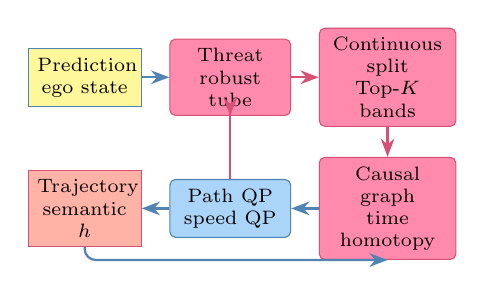
\begin{tikzpicture}[node distance=3.8mm and 3.5mm]
 \node[modin,text width=12mm] (in) {Prediction\\ego state};
 \node[modimp,right=of in,text width=13mm] (tube) {Threat\\robust tube};
 \node[modimp,right=of tube,text width=15mm] (space) {Continuous split\\Top-$K$ bands};
 \node[modimp,below=of space,text width=15mm] (time) {Causal graph\\time homotopy};
 \node[mod,left=of time,text width=13mm] (qp) {Path QP\\speed QP};
 \node[modout,left=of qp,text width=12mm] (out) {Trajectory\\semantic $h$};
 \draw[flow] (in)--(tube); \draw[flowimp] (tube)--(space);
 \draw[flowimp] (space)--(time); \draw[flow] (time)--(qp); \draw[flow] (qp)--(out);
 \draw[flowimp,rounded corners] (qp.north) |- (tube.south);
 \draw[flow,rounded corners] (out.south) |- (time.south);
\end{tikzpicture}
\caption{MIKU wraps discrete homotopy generation and validation around the existing path and speed QPs.}
\label{fig:framework}
\end{figure}

Fig.~\ref{fig:framework} summarizes the pipeline. Apollo-style boundary construction, path optimization, ST mapping, and speed optimization provide the continuous backbone. MIKU contributes the robust constraint representation, spatial/temporal candidate organization, bidirectional information transfer, and receding-horizon consistency.

\subsection{Interaction-Aware Robust Occupancy}

We combine collision imminence, longitudinal overlap, relative velocity, obstacle type, and local interaction density in a normalized threat score
\begin{equation}
 \Theta_i=\sum_{r=1}^{5}w_rf_r(i),\qquad w_r\ge0,\quad\sum_rw_r=1.
 \label{eq:threat}
\end{equation}
The lateral expansion for obstacle $i$ is
\begin{equation}
 \delta_i=\frac{W_e}{2}+d_0+d_\Theta\Theta_i.
 \label{eq:margin}
\end{equation}
Equation~\eqref{eq:road} contracts the physical road into a center-feasible interval, while \eqref{eq:margin} expands each obstacle into a center-forbidden interval; the ego width is therefore counted once at each physical boundary rather than subtracted again from the remaining gap.

For dynamic obstacle $i$, bounded longitudinal and lateral prediction errors grow as
\begin{equation}
 \rho_{q,i}(t)=\rho^0_{q,i}+t\dot\rho_{q,i},\qquad q\in\{s,l\}.
\end{equation}
The robust tube is
\begin{equation}
 O_i^{\rm rob}(t)=O_i(t)\oplus[-\rho_{s,i}(t),\rho_{s,i}(t)]
 \times[-\rho_{l,i}(t),\rho_{l,i}(t)].
 \label{eq:tube}
\end{equation}
The same tube is used by lateral projection, ST mapping, and planning-time safety validation. During ST mapping, MIKU checks the complete lateral envelope of the curved path over the vehicle--obstacle longitudinal Minkowski interval, rather than querying $l(s)$ only at the obstacle center. This prevents missed corner overlap.

\subsection{Continuous Partitions and K-Best Spatial Homotopies}

An initial arrival map $\tau(s)$ queries \eqref{eq:tube} and produces center-forbidden intervals $[u_i(s),v_i(s)]$. A longitudinal sweep divides overlapping obstacles into conflict groups. For a group of $k$ obstacles, sort by nondecreasing $u_i$ and define, for $p=0,\ldots,k$,
\begin{align}
 V_p&=\max\{l^-_{\rm road},v_{(1)},\ldots,v_{(p)}\},\\
 U_p&=\min\{l^+_{\rm road},u_{(p+1)}\},\qquad g_p=U_p-V_p,
 \label{eq:gap}
\end{align}
where empty prefixes and suffixes use the corresponding road bound. Split $p$ places the first $p$ obstacles on one side of the band $[V_p,U_p]$ and the rest on the other.

\begin{lemma}[Continuous partition]
For every feasible binary passing-side assignment, there exists a noninterleaved assignment with no smaller center-feasible width: a prefix of the ordered obstacles lies on one side and the remaining suffix lies on the other.
\label{lem:partition}
\end{lemma}
\begin{proof}
If an assignment contains an inversion in the $u$ order, removing that inversion neither decreases the active upper-bound minimum nor increases the active lower-bound maximum. Repeating the exchange yields one split point without reducing width.
\end{proof}

\begin{theorem}[Exact maximum gap]
The maximum center-feasible width among all $2^k$ passing-side assignments equals
\begin{equation}
 g^*=\max_{p\in\{0,\ldots,k\}}(U_p-V_p).
\end{equation}
It is obtained in $O(k\log k)$ time by sorting, a prefix-maximum scan, and a linear maximum search.
\label{thm:maxgap}
\end{theorem}
\begin{proof}
For split $p$, intersection of all lower-side constraints gives $V_p$, and intersection of all upper-side constraints gives $U_p$. Thus its exact width is $g_p$. Lemma~\ref{lem:partition} guarantees that at least one global optimum is among these $k+1$ splits.
\end{proof}

MIKU ranks every positive-width $[V_p,U_p]$ using width, reference-line displacement, and inter-group center transition. To obtain global alternatives, a layered dynamic program retains the $K$ best prefixes ending at each current band. Future cost depends on a prefix only through its terminal band, so this is an exact K-best procedure for the layered first-order graph. With $M$ groups and at most $Q$ retained bands per group, its complexity is $O(MKQ^2\log(KQ))$. We use $Q=K=3$. Ranked spatial candidates are sent to the QPs until one is certified feasible.

\subsection{Causal Temporal Homotopies and Bidirectional ST Bounds}

For a spatial candidate, intersection with robust tubes yields station-ordered conflicts $c_r=(s_r,\mathcal I_r)$, where $\mathcal I_r$ is a union of occupied time intervals. Connected components of the complement are safe-window nodes. A window before the first occupied interval is labeled \emph{pass-before}; a window after the last interval is \emph{yield-after}; an intermediate window combines yielding to one occupancy and passing before the next.

Two nodes at successive conflict stations are connected only if their candidate arrival times obey
\begin{equation}
 t_b-t_a\ge\frac{s_b-s_a}{v_{\max}}.
 \label{eq:causal}
\end{equation}
The graph cost combines deviation from nominal arrival, waiting, class switching, and receding-horizon persistence. A deterministic beam of width eight returns ranked complete homotopies. For an occupied interval $[t_i^-,t_i^+]$ and longitudinal collision range $[s_i^-,s_i^+]$, the selected class is compiled as
\begin{align}
 \text{pass-before: }&s(t_j)\ge s_i^++\varepsilon_s, &&t_j\ge t_i^+,\label{eq:pass}\\
 \text{yield-after: }&s(t_j)\le s_i^--\varepsilon_s, &&t_j<t_i^-.
 \label{eq:yield}
\end{align}
Equation~\eqref{eq:pass} is an ST lower bound that commits the ego beyond the conflict after the window closes; \eqref{eq:yield} is an upper bound that keeps it before the conflict until the window opens. MIKU validates up to three ranked temporal plans for each spatial plan and stops at the first feasible speed QP.

\begin{proposition}[Convexity preservation]
If the original path and speed objectives are convex quadratic and their dynamics are linear, fixing $(h_l,h_t)$ leaves both subproblems convex QPs.
\end{proposition}
\begin{proof}
Spatial bands and \eqref{eq:pass}--\eqref{eq:yield} are sample-wise affine lower/upper bounds. Their intersection with the original linear constraints is convex and does not change the quadratic Hessian.
\end{proof}

\begin{proposition}[Robust collision exclusion]
If $O_i^{\rm true}(t)\subseteq O_i^{\rm rob}(t)$ and the continuously executed trajectory remains in the corridor constructed by excluding $O_i^{\rm rob}$ and the vehicle footprint, it cannot intersect $O_i^{\rm true}(t)$.
\end{proposition}
\begin{proof}
Disjointness from a superset implies disjointness from every subset.
\end{proof}

\subsection{On-Demand Refinement and Receding-Horizon Consistency}

The first arrival map follows a second-order kinematic estimate. When a purely dynamic conflict makes the first pass infeasible, the speed solution produces a first-arrival inverse $\hat\tau^{(r)}(s)$ and MIKU updates
\begin{equation}
 \tau^{(r+1)}(s)=(1-\alpha)\tau^{(r)}(s)+\alpha\hat\tau^{(r)}(s),
 \qquad \alpha=0.7.
 \label{eq:refinement}
\end{equation}
At most two planning passes are performed, and the best verified feasible iterate is retained. Thus refinement repairs temporal mismatch on demand rather than adding unconditional cycles.

Across receding-horizon cycles, spatial and temporal choices carry semantic labels. Switching labels incurs a persistence cost. Moreover, after selecting a verified pass-before trajectory, MIKU commits to that trajectory until the ego clears the conflict. This prevents an unsafe late switch to yielding after the stopping line has already been crossed.

\begin{algorithm}[t]
\scriptsize
\caption{MIKU Homotopy-Corridor Planning}
\label{alg:miku}
\KwIn{Ego state, road bounds, predicted obstacles, previous labels}
\KwOut{Path $l(s)$, speed $s(t)$, homotopy $h$}
Build threat margins and robust occupancy tubes; initialize $\tau^{(0)}$\;
\For{$r=0,1$}{
 Generate exact K-best spatial homotopies from continuous splits\;
 \ForEach{ranked spatial homotopy}{
  Solve path QP; map the full path envelope to robust ST conflicts\;
  Generate causal temporal homotopies\;
  \ForEach{ranked temporal homotopy}{
   Compile bidirectional ST bounds and solve speed QP\;
   Store every robustly verified feasible trajectory\;
  }
 }
 Stop if feasible or refinement is not triggered; otherwise update \eqref{eq:refinement}\;
}
Return the minimum-cost feasible trajectory and persist its semantic label\;
\end{algorithm}

\section{Experimental Evaluation}
\label{sec:experiments}

\subsection{Protocol}

We compare four methods on the same Apollo-style path--speed chain. B0 uses time-blind static path bounds, a fixed margin, and greedy obstacle-wise nudging. B1 adds arrival-time projection but retains greedy spatial decisions. B2 alternates path and speed timing for up to three iterations. MIKU enables robust occupancy, threat-adaptive margins, grouping, exact K-best spatial homotopies, the temporal graph, bidirectional ST bounds, and on-demand refinement. All methods share scenarios, predictions, vehicle geometry, QPs, dynamics, horizons, and objective weights.

Seven scenario families cover pedestrian crossing, vehicle cut-in, parked vehicle with oncoming traffic, narrow multi-obstacle passages, interleaved dynamic obstacles, noisy prediction, and delayed crossing. Each family uses \RandSeedCount{} fixed seeds, yielding \RandCaseCount{} paired cases. The noisy family perturbs planner inputs while evaluation uses unperturbed truth. A success is a collision-free arrival at the evaluation line within the horizon. Collision is continuous-time overlap of physical ego/obstacle rectangles. Full-cycle latency includes constraint construction, candidate generation, both QPs, and triggered refinements.

Binary outcomes use an exact McNemar test. Percentage-point differences and continuous effects use 5,000 paired bootstrap resamples for 95\% confidence intervals (CIs). The main timing experiment runs methods sequentially in one process on an Intel Core i9-14900HX under Linux 7.2.2 with OSQP 1.1.1 \cite{stellato2020osqp}. Raw cases, failures, statistics, plots, and manuscript macros are produced by one evaluation entry point.

\subsection{Overall Performance}

\begin{table*}[t]
\caption{Aggregate Results Over Seven Randomized Families ($n=\RandCaseCount$ Per Method)}
\label{tab:overall}
\centering
\small
\begin{tabular}{lrrrrrrrr}
\toprule
Method & Success (\%) & Collision (\%) & Stop (\%) & Clearance (m) & Jerk RMS & P50 (ms) & P95 (ms) & P99 (ms)\\
\midrule
B0 & \RandAllBZeroSuccessPct & \RandAllBZeroCollisionPct & \RandAllBZeroStopPct & \RandAllBZeroClearance & \RandAllBZeroJerkRms & \RandAllBZeroRuntimePfifty & \RandAllBZeroRuntimePninetyfive & \RandAllBZeroRuntimePninetynine\\
B1 & \RandAllBOneSuccessPct & \RandAllBOneCollisionPct & \RandAllBOneStopPct & \RandAllBOneClearance & \RandAllBOneJerkRms & \RandAllBOneRuntimePfifty & \RandAllBOneRuntimePninetyfive & \RandAllBOneRuntimePninetynine\\
B2 & \RandAllBTwoSuccessPct & \RandAllBTwoCollisionPct & \RandAllBTwoStopPct & \RandAllBTwoClearance & \RandAllBTwoJerkRms & \RandAllBTwoRuntimePfifty & \RandAllBTwoRuntimePninetyfive & \RandAllBTwoRuntimePninetynine\\
MIKU & \RandAllMikuSuccessPct & \RandAllMikuCollisionPct & \RandAllMikuStopPct & \RandAllMikuClearance & \RandAllMikuJerkRms & \RandAllMikuRuntimePfifty & \RandAllMikuRuntimePninetyfive & \RandAllMikuRuntimePninetynine\\
\bottomrule
\end{tabular}
\end{table*}

MIKU reaches \RandAllMikuSuccessPct\% collision-free success versus \RandAllBZeroSuccessPct\%, \RandAllBOneSuccessPct\%, and \RandAllBTwoSuccessPct\% for B0--B2 (Table~\ref{tab:overall}). The paired MIKU--B0 gain is \RandAllMikuVsBZeroSuccessDiff{} points (95\% CI \RandAllMikuVsBZeroSuccessCiLow--\RandAllMikuVsBZeroSuccessCiHigh; exact McNemar $p=\RandAllMikuVsBZeroSuccessMcNemarP$). Collision falls from \RandAllBZeroCollisionPct\% to \RandAllMikuCollisionPct\%, a paired difference of \RandAllMikuVsBZeroCollisionDiff{} points (95\% CI \RandAllMikuVsBZeroCollisionCiLow--\RandAllMikuVsBZeroCollisionCiHigh; $p=\RandAllMikuVsBZeroCollisionMcNemarP$). The increased traversal capability therefore does not trade against safety.

MIKU's P95 complete-planning latency is \RandAllMikuRuntimePninetyfive\,ms, comparable to B0 at \RandAllBZeroRuntimePninetyfive\,ms and substantially below the unconditional iterative B2 at \RandAllBTwoRuntimePninetyfive\,ms. Its higher P99 reflects on-demand candidate fallback, while the P95 shows that most cases terminate on an early feasible homotopy.

\begin{figure}[t]
\centering
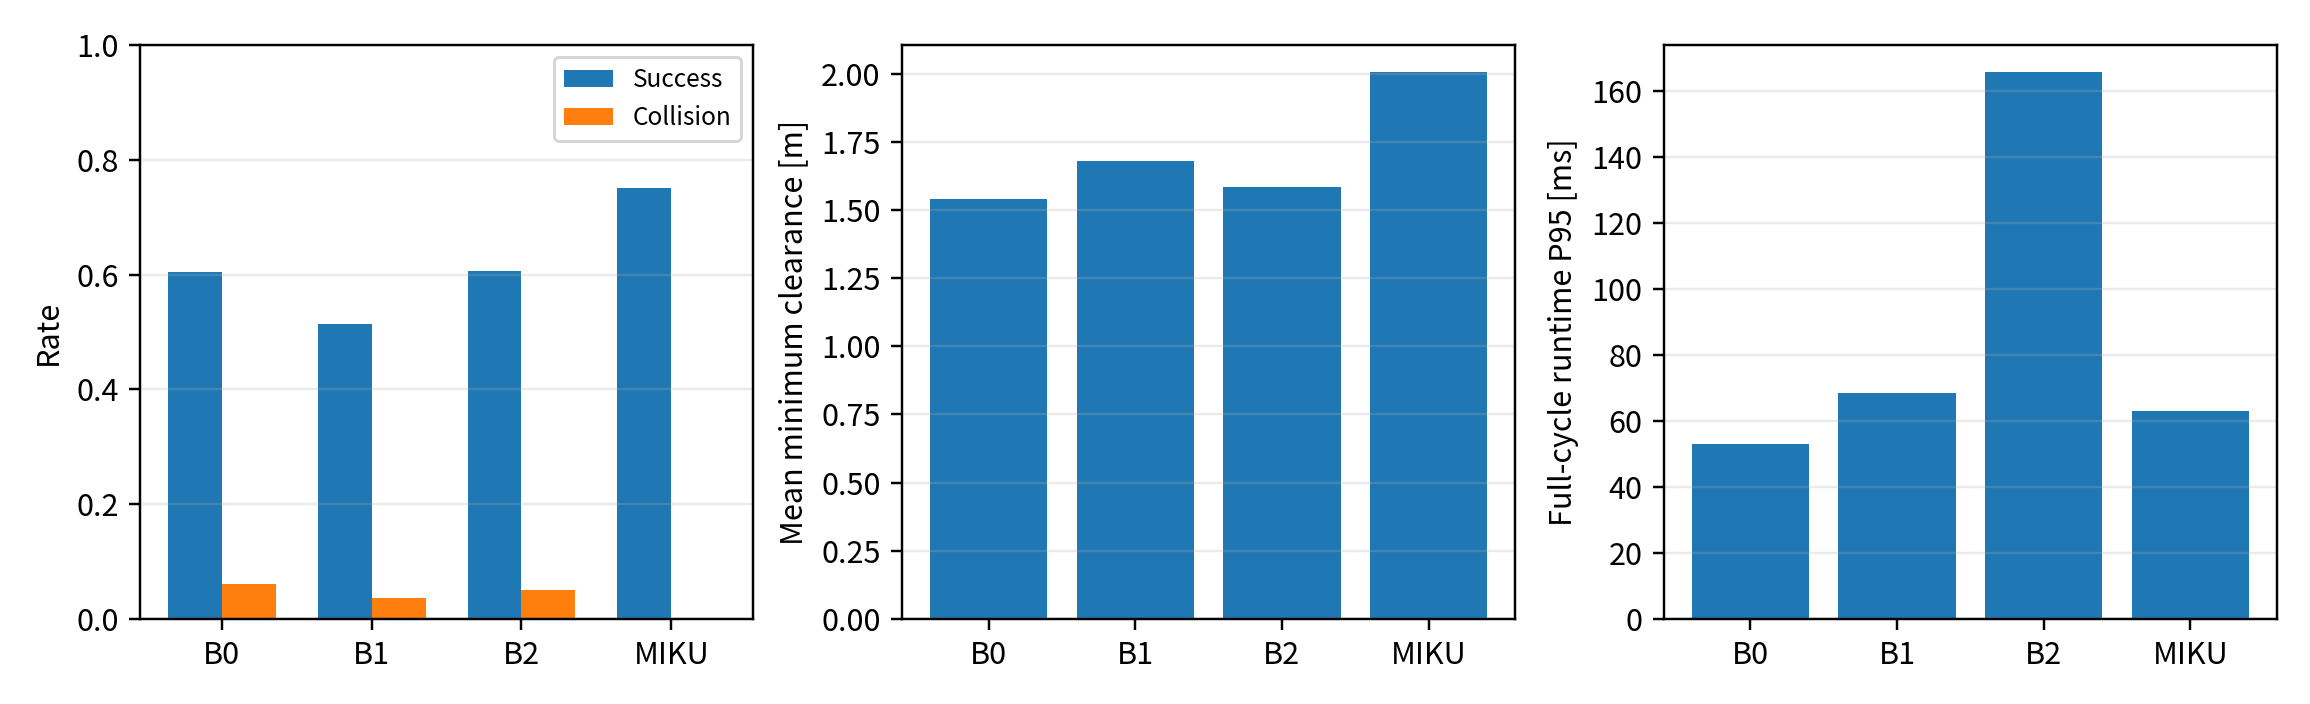
\includegraphics[width=\columnwidth]{generated/randomized_summary.png}
\caption{Aggregate paired-randomized evaluation.}
\label{fig:summary}
\end{figure}

\subsection{Scenario-Wise Effects}

\begin{table}[t]
\caption{MIKU vs. B0 Success by Scenario Family}
\label{tab:family}
\centering
\scriptsize
\begin{tabular}{lrrrr}
\toprule
Family & B0 & MIKU & Diff. & 95\% CI\\
\midrule
Crossing & \RandCrossingBZeroSuccessPct & \RandCrossingMikuSuccessPct & \RandCrossingMikuVsBZeroSuccessDiff & [\RandCrossingMikuVsBZeroSuccessCiLow,\RandCrossingMikuVsBZeroSuccessCiHigh]\\
Cut-in & \RandCutInBZeroSuccessPct & \RandCutInMikuSuccessPct & \RandCutInMikuVsBZeroSuccessDiff & [\RandCutInMikuVsBZeroSuccessCiLow,\RandCutInMikuVsBZeroSuccessCiHigh]\\
Parked/oncoming & \RandParkedBZeroSuccessPct & \RandParkedMikuSuccessPct & \RandParkedMikuVsBZeroSuccessDiff & [\RandParkedMikuVsBZeroSuccessCiLow,\RandParkedMikuVsBZeroSuccessCiHigh]\\
Narrow multi-obs. & \RandNarrowBZeroSuccessPct & \RandNarrowMikuSuccessPct & \RandNarrowMikuVsBZeroSuccessDiff & [\RandNarrowMikuVsBZeroSuccessCiLow,\RandNarrowMikuVsBZeroSuccessCiHigh]\\
Interleaved & \RandInterleavedBZeroSuccessPct & \RandInterleavedMikuSuccessPct & \RandInterleavedMikuVsBZeroSuccessDiff & [\RandInterleavedMikuVsBZeroSuccessCiLow,\RandInterleavedMikuVsBZeroSuccessCiHigh]\\
Prediction noise & \RandNoiseBZeroSuccessPct & \RandNoiseMikuSuccessPct & \RandNoiseMikuVsBZeroSuccessDiff & [\RandNoiseMikuVsBZeroSuccessCiLow,\RandNoiseMikuVsBZeroSuccessCiHigh]\\
Delayed crossing & \RandDelayedBZeroSuccessPct & \RandDelayedMikuSuccessPct & \RandDelayedMikuVsBZeroSuccessDiff & [\RandDelayedMikuVsBZeroSuccessCiLow,\RandDelayedMikuVsBZeroSuccessCiHigh]\\
\bottomrule
\end{tabular}
\end{table}

The largest spatial gain occurs in narrow multi-obstacle passages: \RandNarrowMikuVsBZeroSuccessDiff{} points, consistent with continuous partitions recovering corridors discarded by greedy nudging. Delayed crossing improves by \RandDelayedMikuVsBZeroSuccessDiff{} points, demonstrating the value of explicit pass-before/yield-after choices. Under prediction noise, success improves by \RandNoiseMikuVsBZeroSuccessDiff{} points and collision changes by \RandNoiseMikuVsBZeroCollisionDiff{} points, directly supporting robust-tube propagation. Crossing and interleaved cases are already near saturation for B0, and MIKU maintains their success.

\subsection{Large-Scale Paired Ablation}

Each ablation uses the same seven families and \RandCaseCount{} paired seeds. A1 removes arrival-time initialization, A2 grouping, A3 K-best spatial homotopy, A4 threat-adaptive margins, A5 the temporal graph, A6 robust occupancy, and A7 alternating refinement. Differences in Table~\ref{tab:ablation} are full MIKU minus the ablation.

\begin{table*}[t]
\caption{Paired Component Ablation Over \RandCaseCount Cases}
\label{tab:ablation}
\centering
\small
\begin{tabular}{lrrrrr}
\toprule
Configuration & Success (\%) & Collision (\%) & Gain (points) & 95\% CI & McNemar $p$\\
\midrule
Full MIKU & \AblMikuSuccessPct & \AblMikuCollisionPct & --- & --- & ---\\
A1 w/o arrival initialization & \AblAOneSuccessPct & \AblAOneCollisionPct & \AblMikuVsAOneSuccessDiff & [\AblMikuVsAOneSuccessCiLow,\AblMikuVsAOneSuccessCiHigh] & \AblMikuVsAOneSuccessMcNemarP\\
A2 w/o grouping & \AblATwoSuccessPct & \AblATwoCollisionPct & \AblMikuVsATwoSuccessDiff & [\AblMikuVsATwoSuccessCiLow,\AblMikuVsATwoSuccessCiHigh] & \AblMikuVsATwoSuccessMcNemarP\\
A3 w/o K-best spatial homotopy & \AblAThreeSuccessPct & \AblAThreeCollisionPct & \AblMikuVsAThreeSuccessDiff & [\AblMikuVsAThreeSuccessCiLow,\AblMikuVsAThreeSuccessCiHigh] & \AblMikuVsAThreeSuccessMcNemarP\\
A4 w/o threat margin & \AblAFourSuccessPct & \AblAFourCollisionPct & \AblMikuVsAFourSuccessDiff & [\AblMikuVsAFourSuccessCiLow,\AblMikuVsAFourSuccessCiHigh] & \AblMikuVsAFourSuccessMcNemarP\\
A5 w/o temporal graph & \AblAFiveSuccessPct & \AblAFiveCollisionPct & \AblMikuVsAFiveSuccessDiff & [\AblMikuVsAFiveSuccessCiLow,\AblMikuVsAFiveSuccessCiHigh] & \AblMikuVsAFiveSuccessMcNemarP\\
A6 w/o robust occupancy & \AblASixSuccessPct & \AblASixCollisionPct & \AblMikuVsASixSuccessDiff & [\AblMikuVsASixSuccessCiLow,\AblMikuVsASixSuccessCiHigh] & \AblMikuVsASixSuccessMcNemarP\\
A7 w/o refinement & \AblASevenSuccessPct & \AblASevenCollisionPct & \AblMikuVsASevenSuccessDiff & [\AblMikuVsASevenSuccessCiLow,\AblMikuVsASevenSuccessCiHigh] & \AblMikuVsASevenSuccessMcNemarP\\
\bottomrule
\end{tabular}
\end{table*}

K-best spatial homotopy and threat-adaptive margins contribute \AblMikuVsAThreeSuccessDiff{} and \AblMikuVsAFourSuccessDiff{} points, respectively. The temporal graph adds \AblMikuVsAFiveSuccessDiff{} points. Removing robust occupancy increases collision from \AblMikuCollisionPct\% to \AblASixCollisionPct\%; the paired collision difference is \AblMikuVsASixCollisionDiff{} points ($p=\AblMikuVsASixCollisionMcNemarP$). Refinement adds \AblMikuVsASevenSuccessDiff{} points. A1 is not significant, indicating that kinematic arrival time is primarily an initializer; the final benefit arises from homotopy search, QP validation, and feedback refinement.

\subsection{Receding-Horizon and Joint-Reference Evaluation}

The receding-horizon protocol repeatedly plans, executes 0.5\,s, updates ego and obstacles, and replans. It contains 100 seeds per family, or \ClosedCaseCount{} paired episodes. MIKU reaches \ClosedMikuSuccessPct\% versus B0's \ClosedBZeroSuccessPct\%, a \ClosedMikuVsBZeroSuccessDiff-point gain (95\% CI \ClosedMikuVsBZeroSuccessCiLow--\ClosedMikuVsBZeroSuccessCiHigh; $p=\ClosedMikuVsBZeroSuccessMcNemarP$). Both collision rates are \ClosedMikuCollisionPct\%. Semantic persistence and pass-before commitment therefore carry the open-loop benefit into repeated replanning without increasing collision.

The B3 reference jointly searches $(t,s,l,v,\dot l)$ on a coarse grid and uses the same threat margins and robust prediction tubes as MIKU. It is a quality--cost reference, not a continuous global optimum. Across \JointCaseCount{} paired cases, B3 and MIKU achieve \JointBThreeSuccessPct\% and \JointMikuSuccessPct\%; the MIKU--B3 difference is \JointMikuVsBThreeSuccessDiff{} points (95\% CI \JointMikuVsBThreeSuccessCiLow--\JointMikuVsBThreeSuccessCiHigh; $p=\JointMikuVsBThreeSuccessMcNemarP$). Thus success is statistically indistinguishable at this sample size. B3's P95 is \JointBThreeRuntimePninetyfive\,ms versus \JointMikuRuntimePninetyfive\,ms for MIKU, showing that finite homotopies plus convex QPs recover comparable feasibility at over two orders of magnitude lower computation. B3 has lower penalized travel time among its solutions, reflecting the remaining efficiency advantage of joint search.

\begin{table}[t]
\caption{Receding-Horizon and Joint-Grid Protocols}
\label{tab:supplement}
\centering
\scriptsize
\begin{tabular}{llrrr}
\toprule
Protocol & Method & Success & Collision & P95 ms\\
\midrule
Rolling ($n=\ClosedCaseCount$) & B0 & \ClosedBZeroSuccessPct & \ClosedBZeroCollisionPct & \ClosedBZeroRuntimePninetyfive\\
 & MIKU & \ClosedMikuSuccessPct & \ClosedMikuCollisionPct & \ClosedMikuRuntimePninetyfive\\
Joint ($n=\JointCaseCount$) & B3 & \JointBThreeSuccessPct & \JointBThreeCollisionPct & \JointBThreeRuntimePninetyfive\\
 & MIKU & \JointMikuSuccessPct & \JointMikuCollisionPct & \JointMikuRuntimePninetyfive\\
\bottomrule
\end{tabular}
\end{table}

\subsection{Sensitivity and Scope}

Perturbing all five threat weights by $\pm\SensPerturbPct\%$ and renormalizing changes the resulting margin by at most \SensWorstRelDev\%. Twenty full-planning perturbations in each of four representative scenarios (80 trajectories total) all succeed; the maximum lateral trajectory deviation is 0.011\,m. The core effect is therefore locally stable rather than dependent on one exact weight vector.

The evaluation covers planner-in-the-loop structured-road scenarios and bounded prediction perturbations. It does not yet include perception false detections, complex intersection rules, or physical actuator errors. These are the next interfaces for probabilistic prediction and vehicle experiments, while the reported theorem, convexity property, executable implementation, and paired simulation evidence remain directly reproducible.

\section{Conclusion}

MIKU introduces an interaction-aware spatiotemporal homotopy corridor around a mature decoupled path--speed solver. A continuous-partition theorem converts $2^k$ passing-side assignments into $k+1$ exact lateral bands; an exact K-best layered search preserves spatial alternatives; and a causal temporal graph compiles pass-before/yield-after orders into bidirectional ST bounds. Robust occupancy, envelope-aware mapping, on-demand refinement, and semantic commitment complete the planning loop while every fixed-homotopy problem remains a convex QP.

Across \RandCaseCount{} paired random cases, MIKU improves collision-free arrival by \RandAllMikuVsBZeroSuccessDiff{} points and reduces collision by 1.0 point relative to B0, with P95 full-planning latency of \RandAllMikuRuntimePninetyfive\,ms. The \ClosedCaseCount-episode receding-horizon study preserves a \ClosedMikuVsBZeroSuccessDiff-point arrival gain. These results establish MIKU as a practical route to richer spatiotemporal decisions without replacing an existing path--velocity optimization stack.

\printbibliography
\end{document}
